\documentclass[]{book}
\usepackage{lmodern}
\usepackage{amssymb,amsmath}
\usepackage{ifxetex,ifluatex}
\usepackage{fixltx2e} % provides \textsubscript
\ifnum 0\ifxetex 1\fi\ifluatex 1\fi=0 % if pdftex
  \usepackage[T1]{fontenc}
  \usepackage[utf8]{inputenc}
\else % if luatex or xelatex
  \ifxetex
    \usepackage{mathspec}
  \else
    \usepackage{fontspec}
  \fi
  \defaultfontfeatures{Ligatures=TeX,Scale=MatchLowercase}
\fi
% use upquote if available, for straight quotes in verbatim environments
\IfFileExists{upquote.sty}{\usepackage{upquote}}{}
% use microtype if available
\IfFileExists{microtype.sty}{%
\usepackage{microtype}
\UseMicrotypeSet[protrusion]{basicmath} % disable protrusion for tt fonts
}{}
\usepackage{hyperref}
\hypersetup{unicode=true,
            pdftitle={GuilStat Performance Management},
            pdfborder={0 0 0},
            breaklinks=true}
\urlstyle{same}  % don't use monospace font for urls
\usepackage{natbib}
\bibliographystyle{apalike}
\usepackage{longtable,booktabs}
\usepackage{graphicx,grffile}
\makeatletter
\def\maxwidth{\ifdim\Gin@nat@width>\linewidth\linewidth\else\Gin@nat@width\fi}
\def\maxheight{\ifdim\Gin@nat@height>\textheight\textheight\else\Gin@nat@height\fi}
\makeatother
% Scale images if necessary, so that they will not overflow the page
% margins by default, and it is still possible to overwrite the defaults
% using explicit options in \includegraphics[width, height, ...]{}
\setkeys{Gin}{width=\maxwidth,height=\maxheight,keepaspectratio}
\IfFileExists{parskip.sty}{%
\usepackage{parskip}
}{% else
\setlength{\parindent}{0pt}
\setlength{\parskip}{6pt plus 2pt minus 1pt}
}
\setlength{\emergencystretch}{3em}  % prevent overfull lines
\providecommand{\tightlist}{%
  \setlength{\itemsep}{0pt}\setlength{\parskip}{0pt}}
\setcounter{secnumdepth}{5}
% Redefines (sub)paragraphs to behave more like sections
\ifx\paragraph\undefined\else
\let\oldparagraph\paragraph
\renewcommand{\paragraph}[1]{\oldparagraph{#1}\mbox{}}
\fi
\ifx\subparagraph\undefined\else
\let\oldsubparagraph\subparagraph
\renewcommand{\subparagraph}[1]{\oldsubparagraph{#1}\mbox{}}
\fi

%%% Use protect on footnotes to avoid problems with footnotes in titles
\let\rmarkdownfootnote\footnote%
\def\footnote{\protect\rmarkdownfootnote}

%%% Change title format to be more compact
\usepackage{titling}

% Create subtitle command for use in maketitle
\providecommand{\subtitle}[1]{
  \posttitle{
    \begin{center}\large#1\end{center}
    }
}

\setlength{\droptitle}{-2em}

  \title{GuilStat Performance Management}
    \pretitle{\vspace{\droptitle}\centering\huge}
  \posttitle{\par}
  \subtitle{Guilford County Operational Metrics}
  \author{true}
    \preauthor{\centering\large\emph}
  \postauthor{\par}
      \predate{\centering\large\emph}
  \postdate{\par}
    \date{2019-10-11}

\usepackage{booktabs}

\begin{document}
\maketitle

{
\setcounter{tocdepth}{1}
\tableofcontents
}
\hypertarget{welcome}{%
\chapter*{Welcome}\label{welcome}}
\addcontentsline{toc}{chapter}{Welcome}

\hypertarget{introduction}{%
\chapter*{Introduction}\label{introduction}}
\addcontentsline{toc}{chapter}{Introduction}

This space would be reserved for a full introduction to the performance management framework and the connection to the strategy framework.

Term definitions should also be provided.

\hypertarget{term-definitions}{%
\chapter*{Term Definitions}\label{term-definitions}}
\addcontentsline{toc}{chapter}{Term Definitions}

\hypertarget{process}{%
\chapter*{Process}\label{process}}
\addcontentsline{toc}{chapter}{Process}

\hypertarget{document-overview}{%
\chapter*{Document Overview}\label{document-overview}}
\addcontentsline{toc}{chapter}{Document Overview}

\hypertarget{enterprise-operational-metrics}{%
\section*{Enterprise Operational Metrics}\label{enterprise-operational-metrics}}
\addcontentsline{toc}{section}{Enterprise Operational Metrics}

\hypertarget{service-areas}{%
\section*{Service Areas}\label{service-areas}}
\addcontentsline{toc}{section}{Service Areas}

\hypertarget{department-operational-metrics}{%
\section*{Department Operational Metrics}\label{department-operational-metrics}}
\addcontentsline{toc}{section}{Department Operational Metrics}

\hypertarget{eoms}{%
\chapter{Enterprise Metrics}\label{eoms}}

This section would be reserved for an overview of Enterprise Operational Metrics.

\hypertarget{dollars-spent-on-overtime}{%
\section{Dollars Spent on Overtime}\label{dollars-spent-on-overtime}}

\hypertarget{overtime-hours-paid}{%
\section{Overtime Hours Paid}\label{overtime-hours-paid}}

\hypertarget{hours-not-worked}{%
\section{Hours Not Worked}\label{hours-not-worked}}

\hypertarget{hours-lost-due-to-work-related-illness-and-injury}{%
\section{Hours Lost Due to Work Related Illness and Injury}\label{hours-lost-due-to-work-related-illness-and-injury}}

\hypertarget{lost-time-injury-rate}{%
\section{Lost Time Injury Rate}\label{lost-time-injury-rate}}

\hypertarget{public-safety}{%
\chapter*{Public Safety}\label{public-safety}}
\addcontentsline{toc}{chapter}{Public Safety}

Guilford County's Public Safety departments work to safeguard and ensure the well-being of residents and visitors. The County addresses public safety in a variety of ways, whether is it through the provision of emergency medical transportation in times of crisis, animal control services or the enforcement of criminal and civil laws and ordinances. All of Guilford County's public safety activities are organized to safeguard our residents' and visitors' well-being.

Public Safety departments include:

\begin{itemize}
\tightlist
\item
  Animal Services
\item
  Emergency Services
\item
  Law Enforcement
\item
  Family Justice Center
\item
  Court Alternatives
\item
  Inspections
\item
  Other Protection
\item
  Security
\end{itemize}

\hypertarget{animalservices}{%
\chapter{Animal Services}\label{animalservices}}

Guilford County Animal Services is responsible for general animal control, regulation and enforcement of animal-related ordinances in the County as well as preventing the occurrence and spread of rabies. Animals that are lost and/or seized are secured and cared for at the Animal Shelter while Animal Control manages rabies prevention programs, responds to vicious animals and animal cruelty, issues warrants and citations to violators, and seizes animals from owners found in violation.

\hypertarget{monthly-call-volume}{%
\section{Monthly Call Volume}\label{monthly-call-volume}}

How many calls do we receive each month?

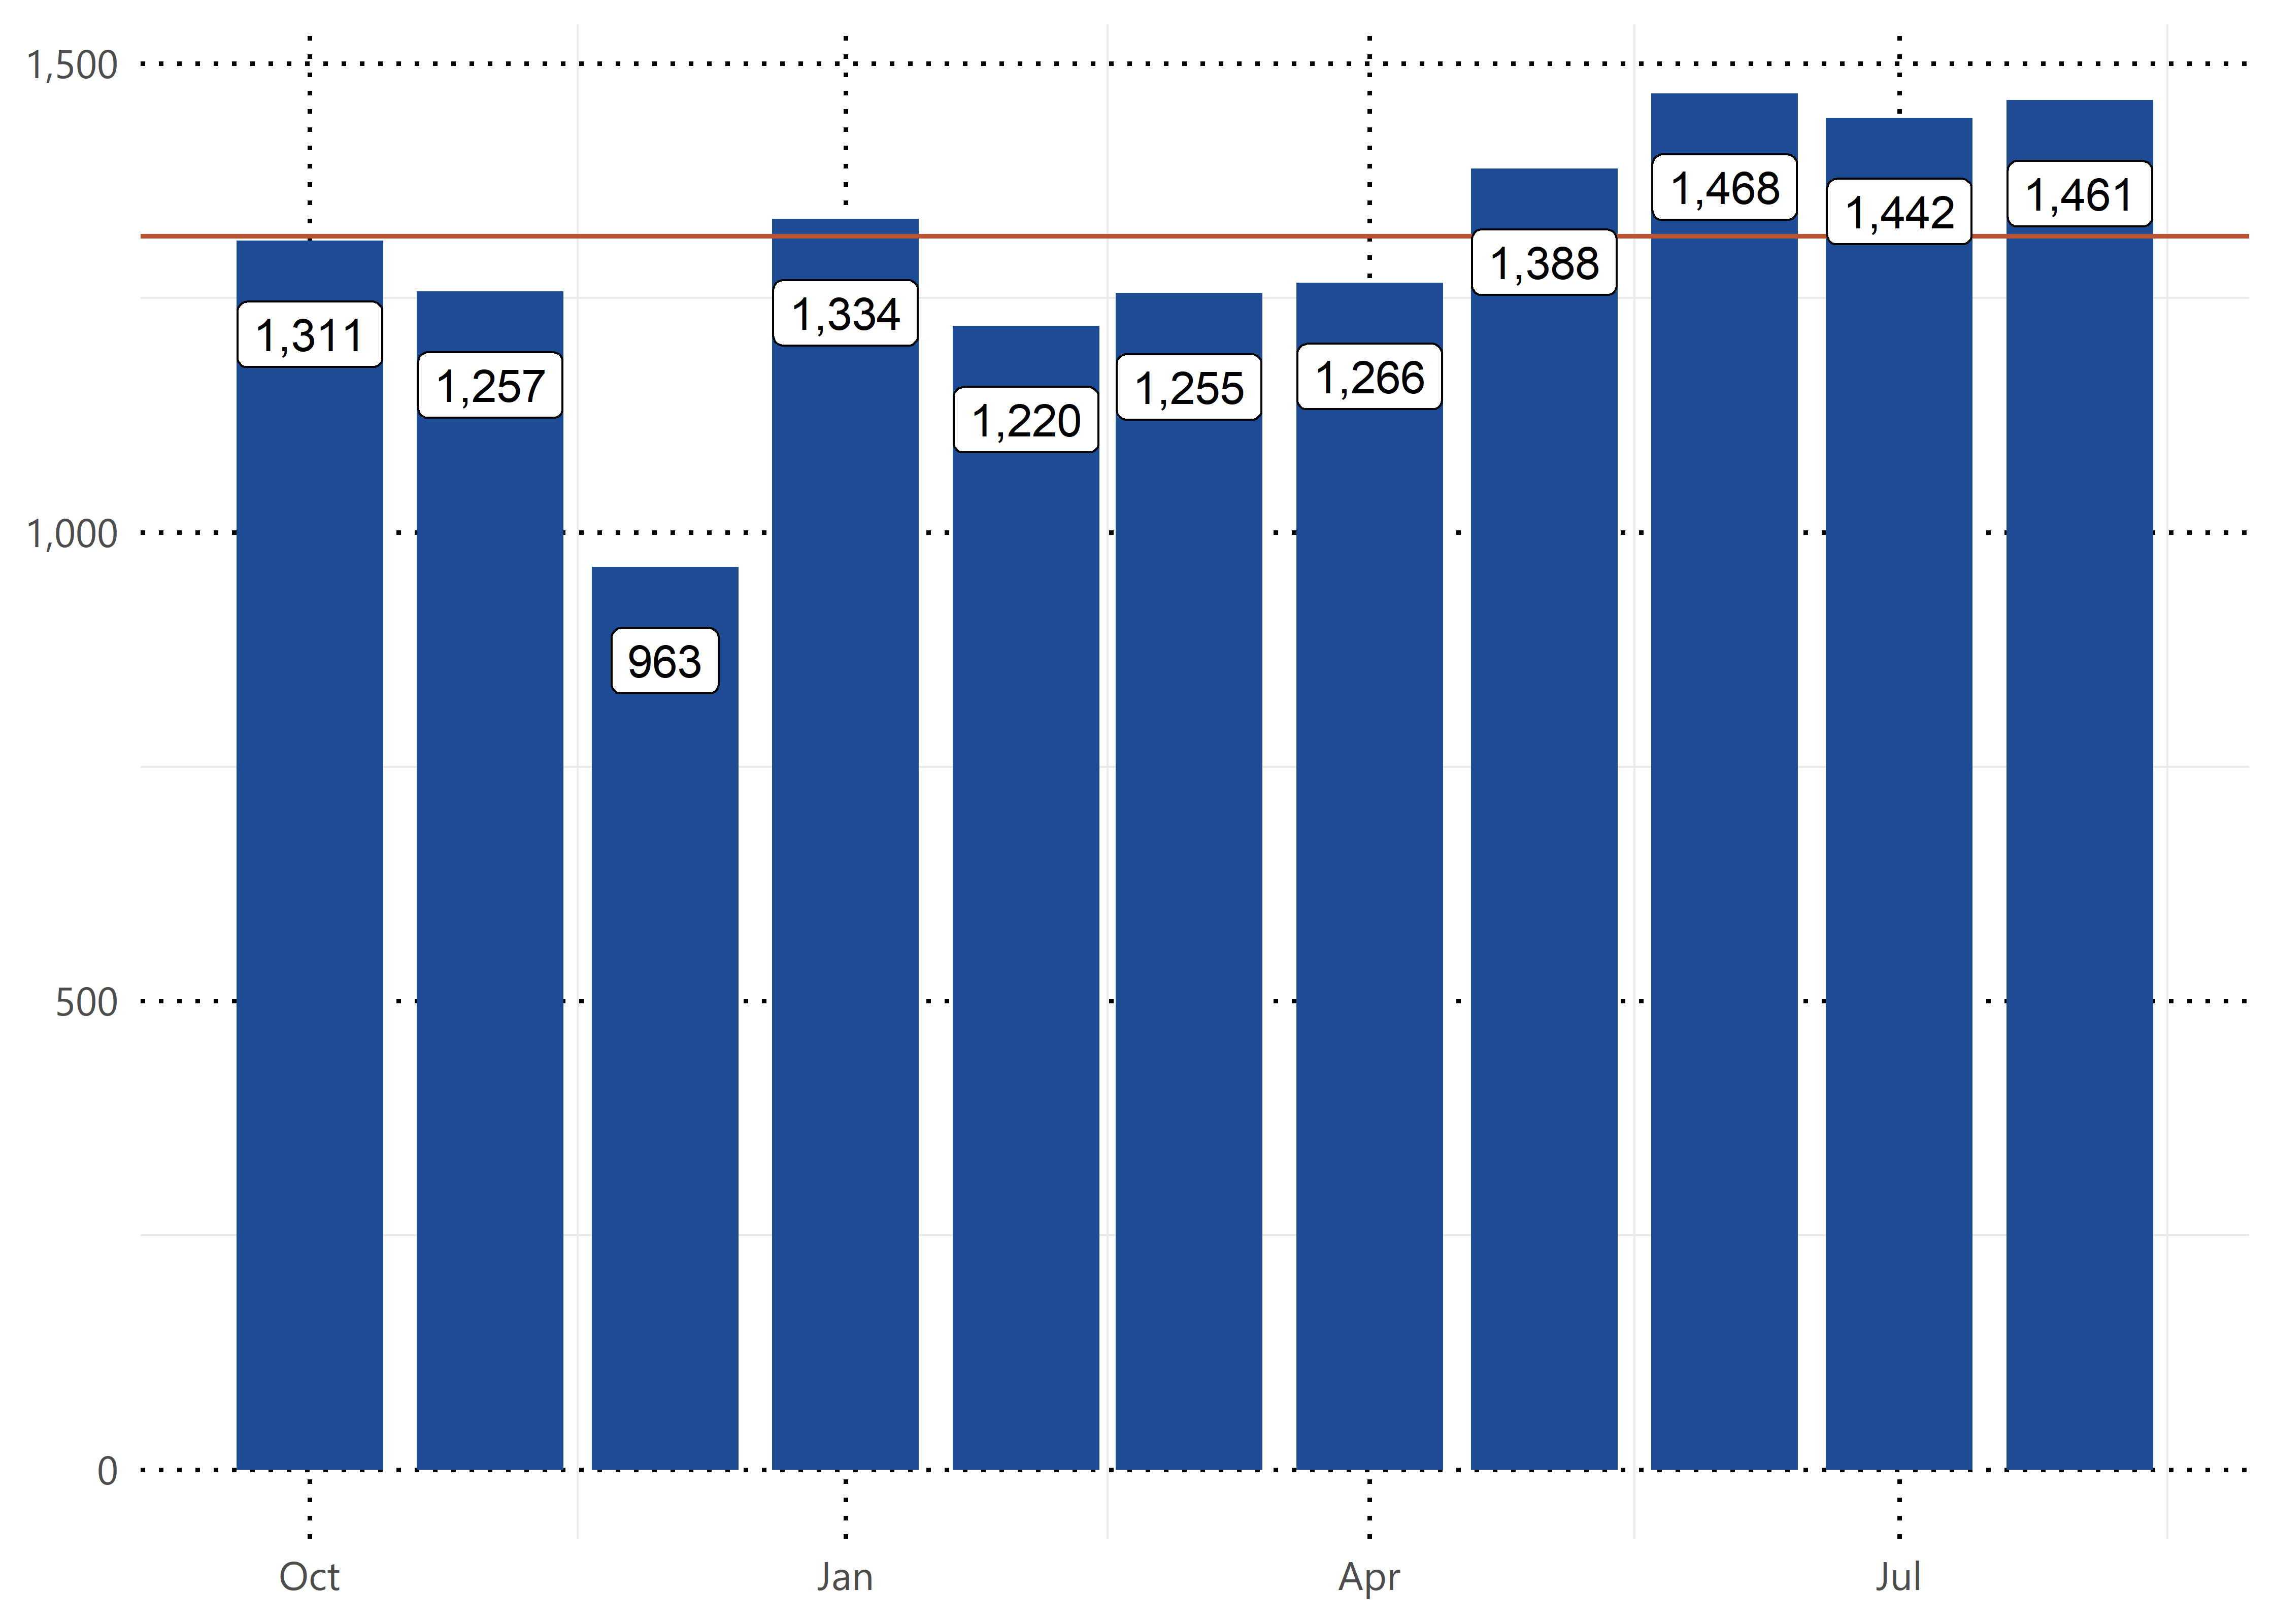
\includegraphics[width=1\linewidth]{bookdown-testing_files/figure-latex/unnamed-chunk-3-1}

\hypertarget{overall-average-response-time}{%
\section{Overall Average Response Time}\label{overall-average-response-time}}

What's our average response time for all calls? Our CAD systems tracks this in seconds so this metric is displayed in seconds.

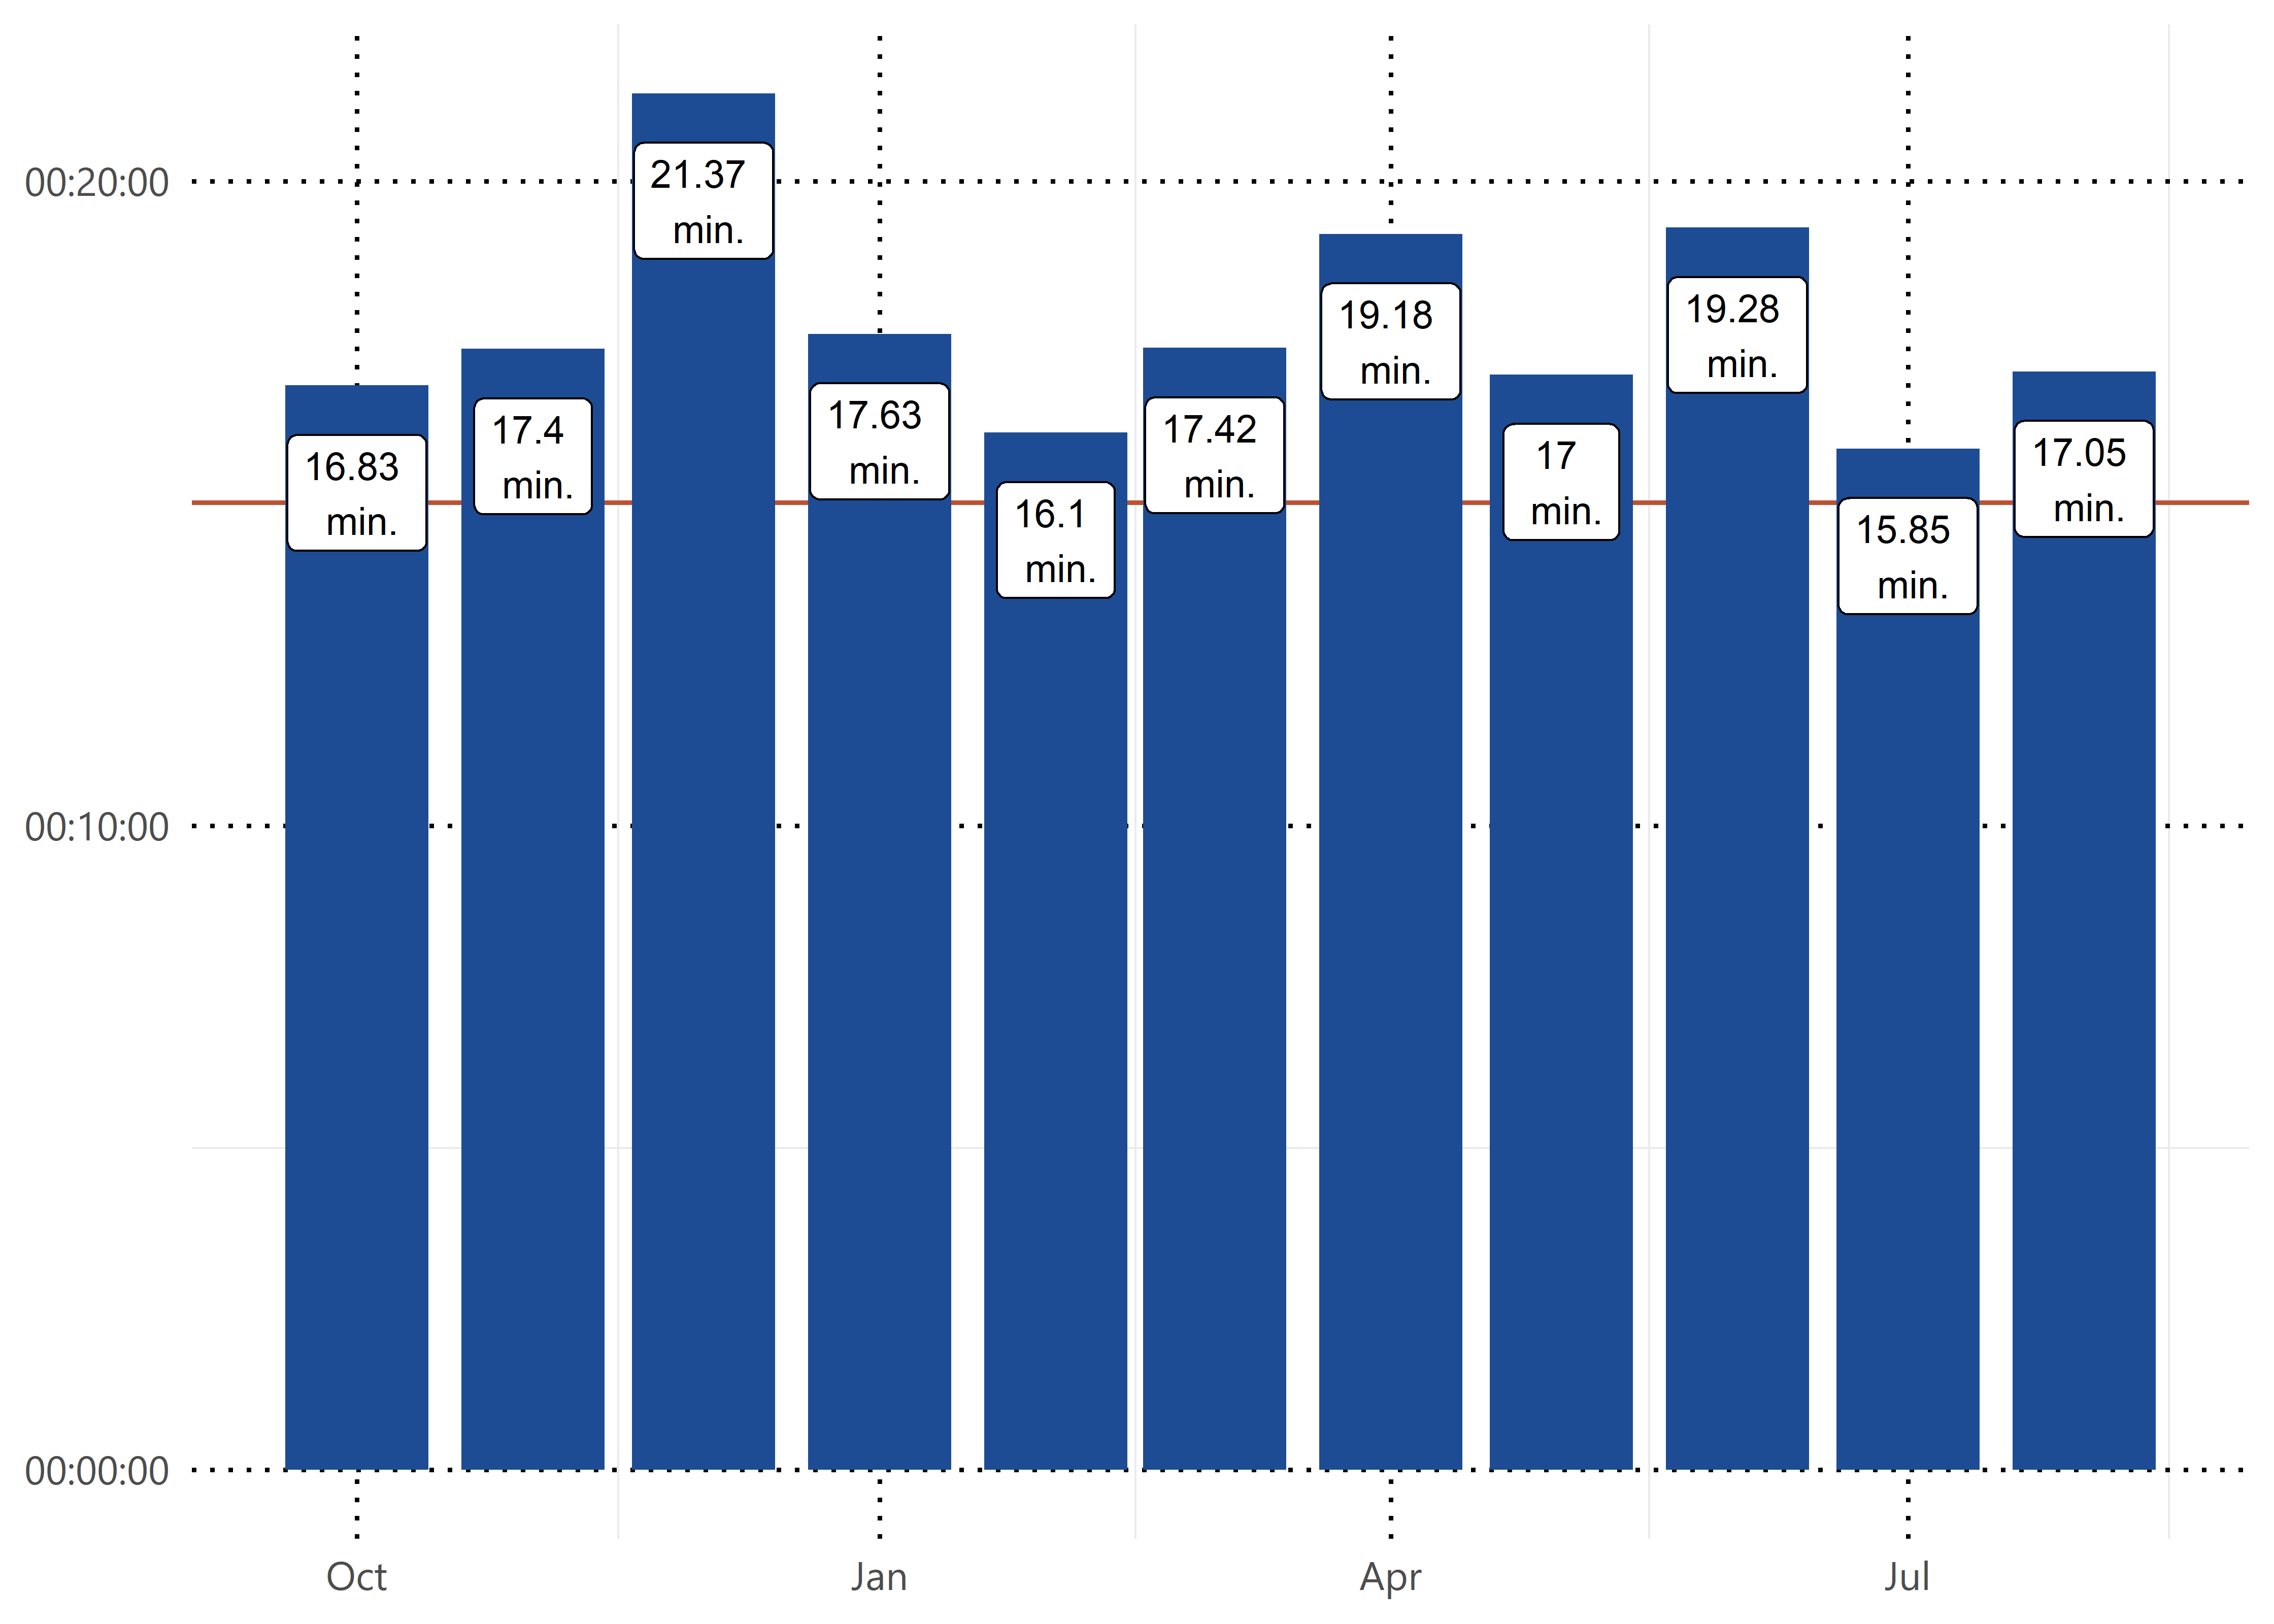
\includegraphics[width=1\linewidth]{bookdown-testing_files/figure-latex/unnamed-chunk-4-1}

\hypertarget{average-response-time-by-jurisdiction}{%
\section{Average Response Time by Jurisdiction}\label{average-response-time-by-jurisdiction}}

What is our average response time broken down by jurisdiction for the most recent month of available data?

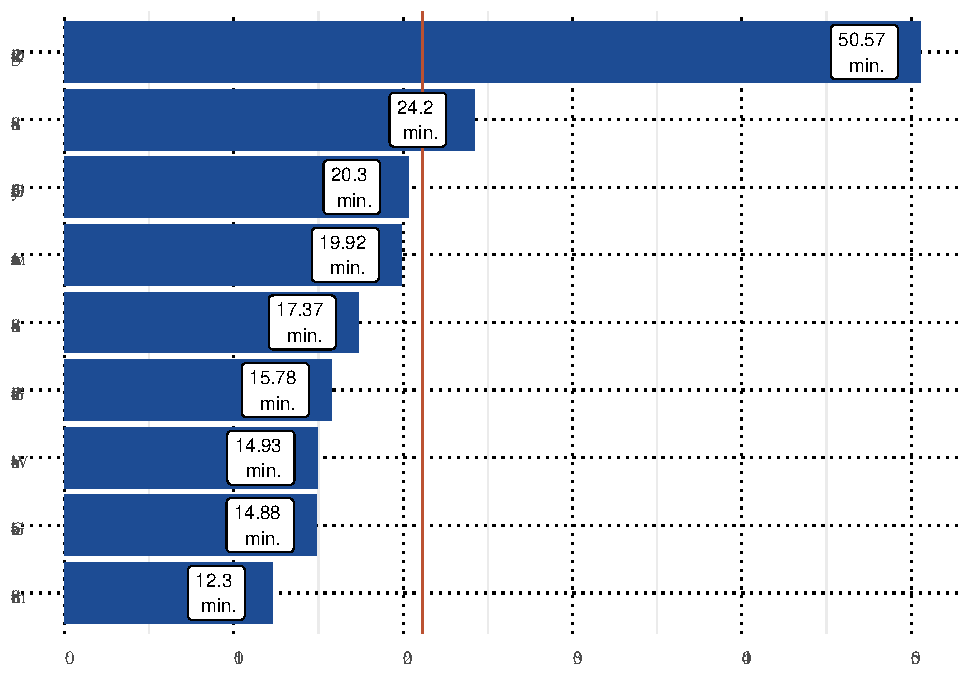
\includegraphics[width=1\linewidth]{bookdown-testing_files/figure-latex/unnamed-chunk-5-1}

\hypertarget{average-response-time-by-day}{%
\section{Average Response Time by Day}\label{average-response-time-by-day}}

What is our average response time broken down by day of the week for the most recent month of available data?

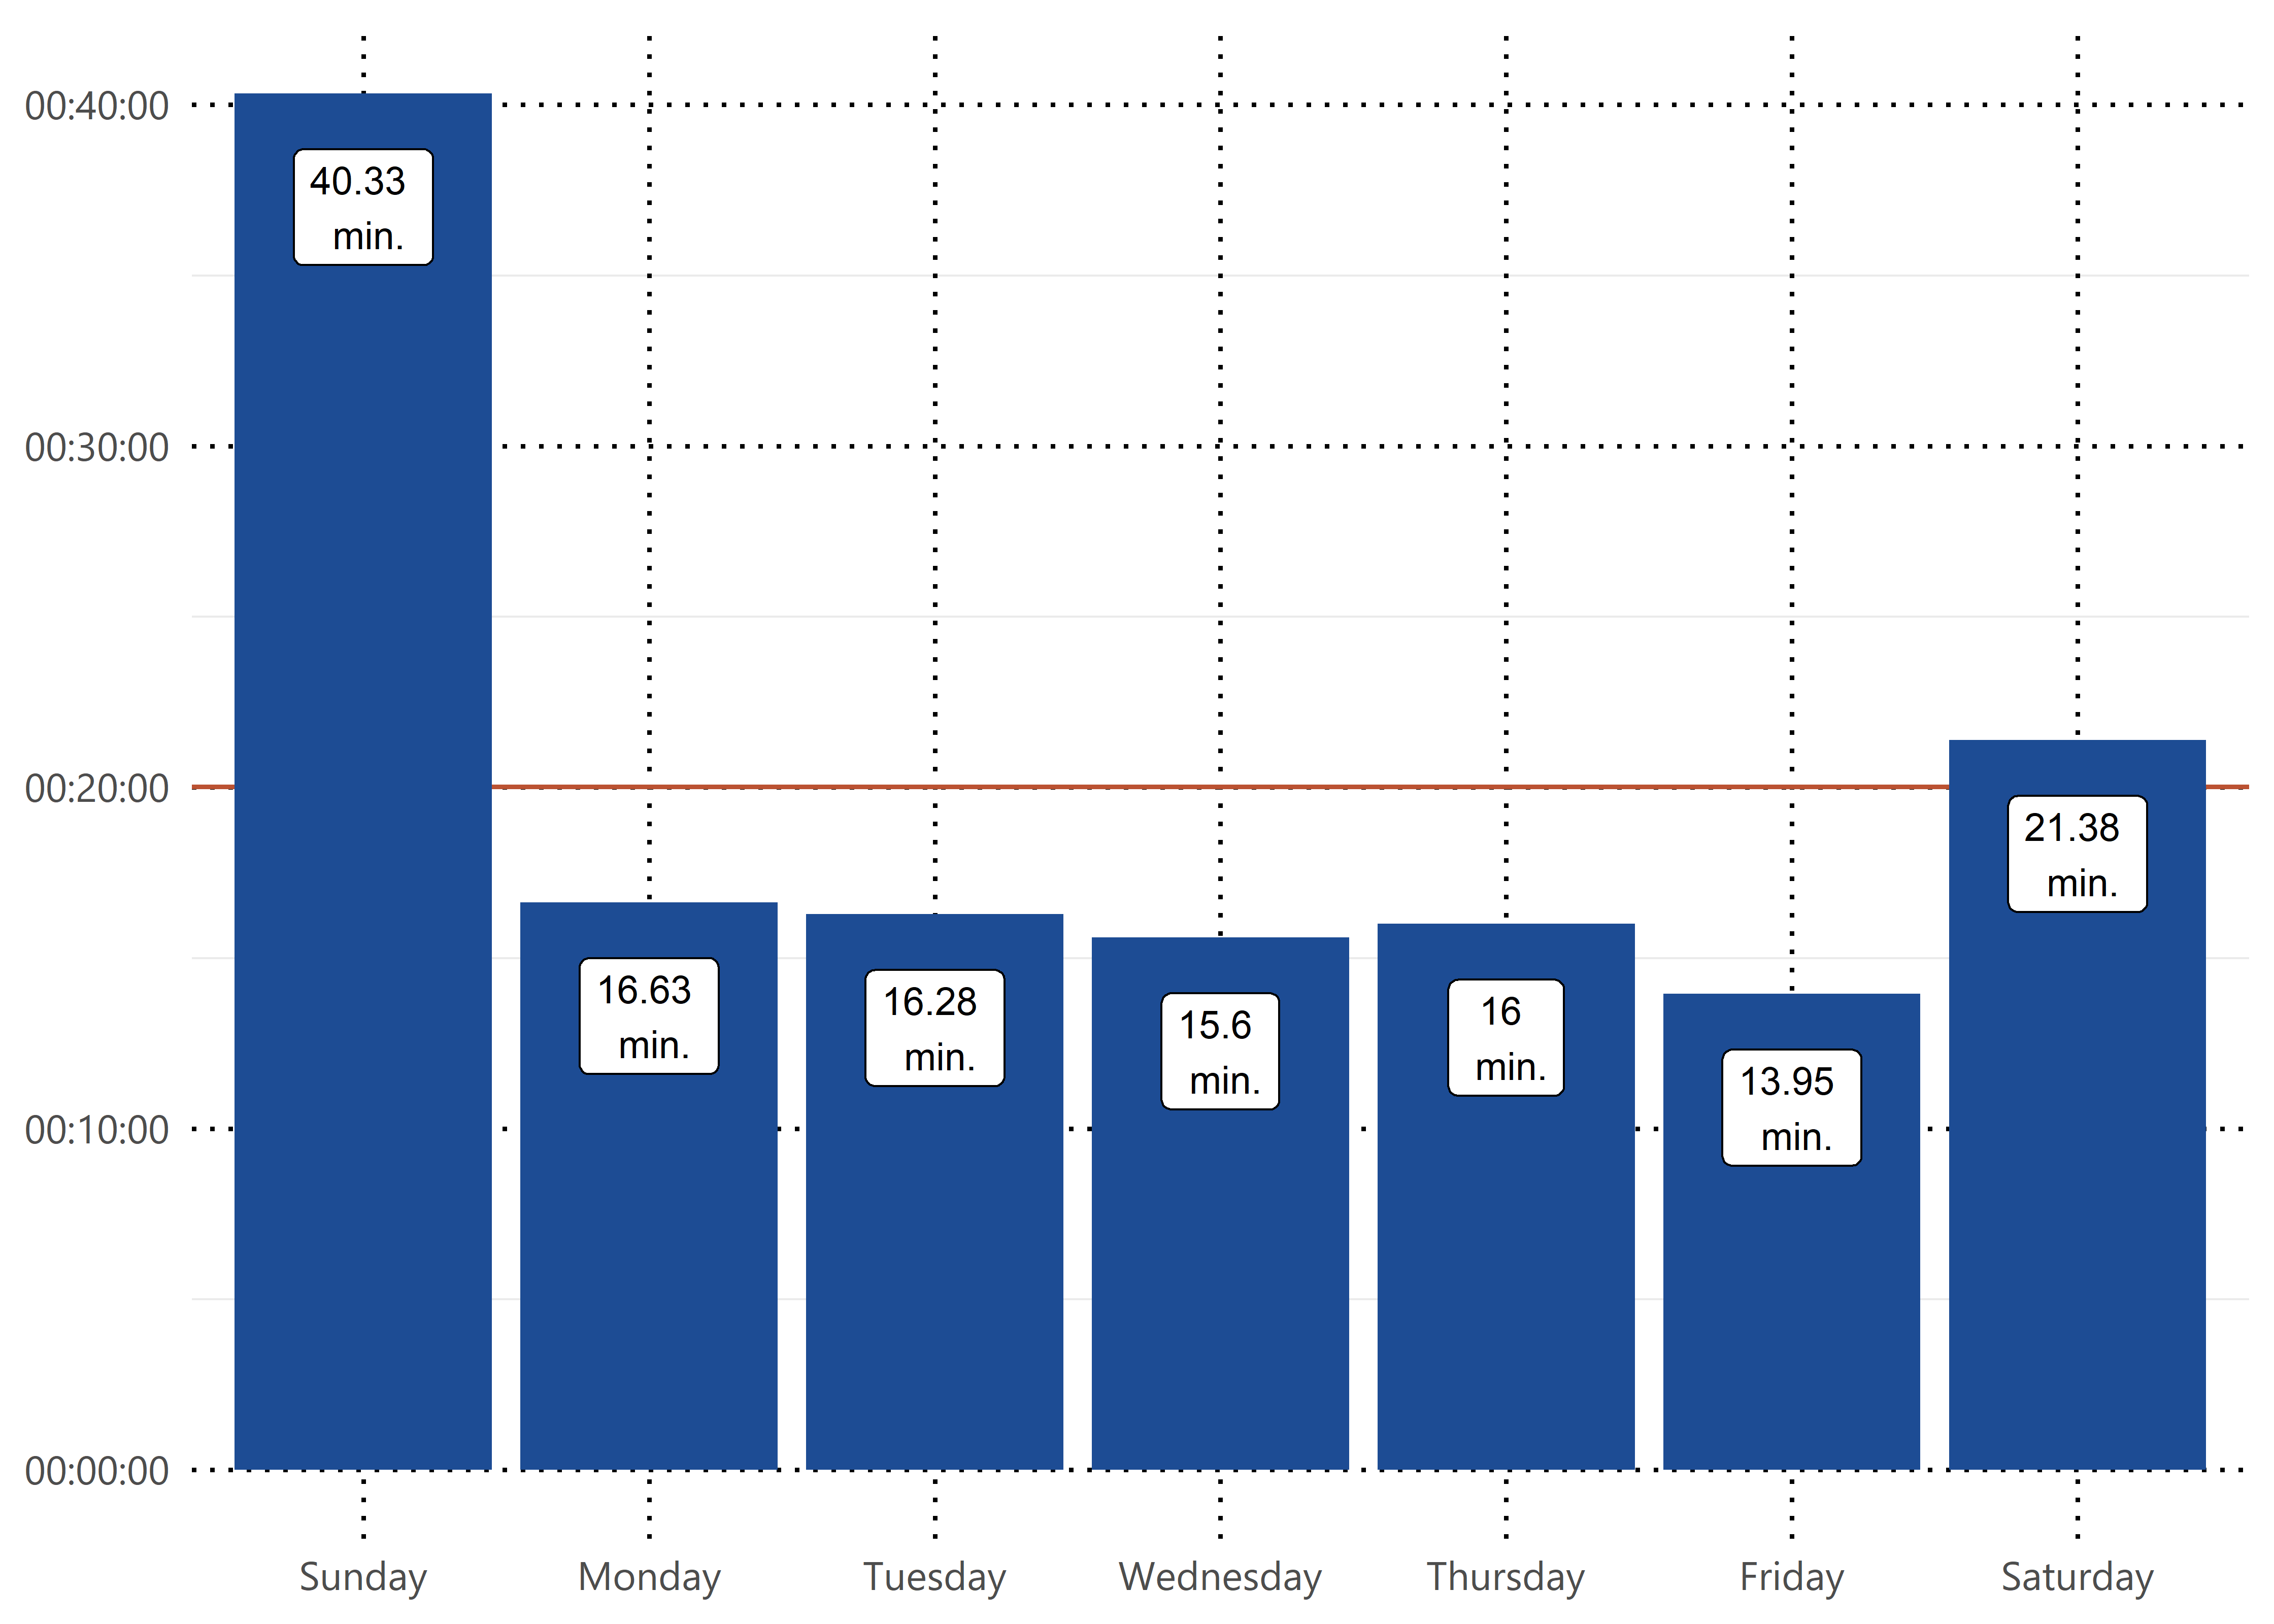
\includegraphics[width=1\linewidth]{bookdown-testing_files/figure-latex/unnamed-chunk-6-1}

\hypertarget{priority-breakdown}{%
\section*{Priority Breakdown}\label{priority-breakdown}}
\addcontentsline{toc}{section}{Priority Breakdown}

Now we will break the calls down into priority designations.

\hypertarget{first-priority-call-volume}{%
\section{First Priority Call Volume}\label{first-priority-call-volume}}

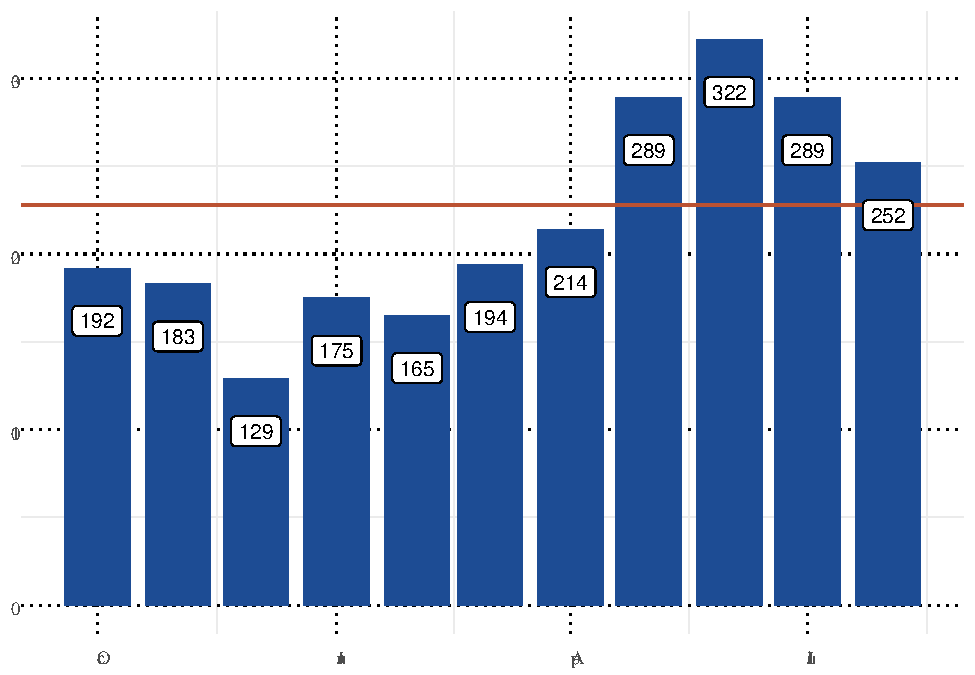
\includegraphics[width=1\linewidth]{bookdown-testing_files/figure-latex/unnamed-chunk-7-1}

\hypertarget{first-priority-average-response-time}{%
\section{First Priority Average Response Time}\label{first-priority-average-response-time}}

Average response time against our established 30 minute target.

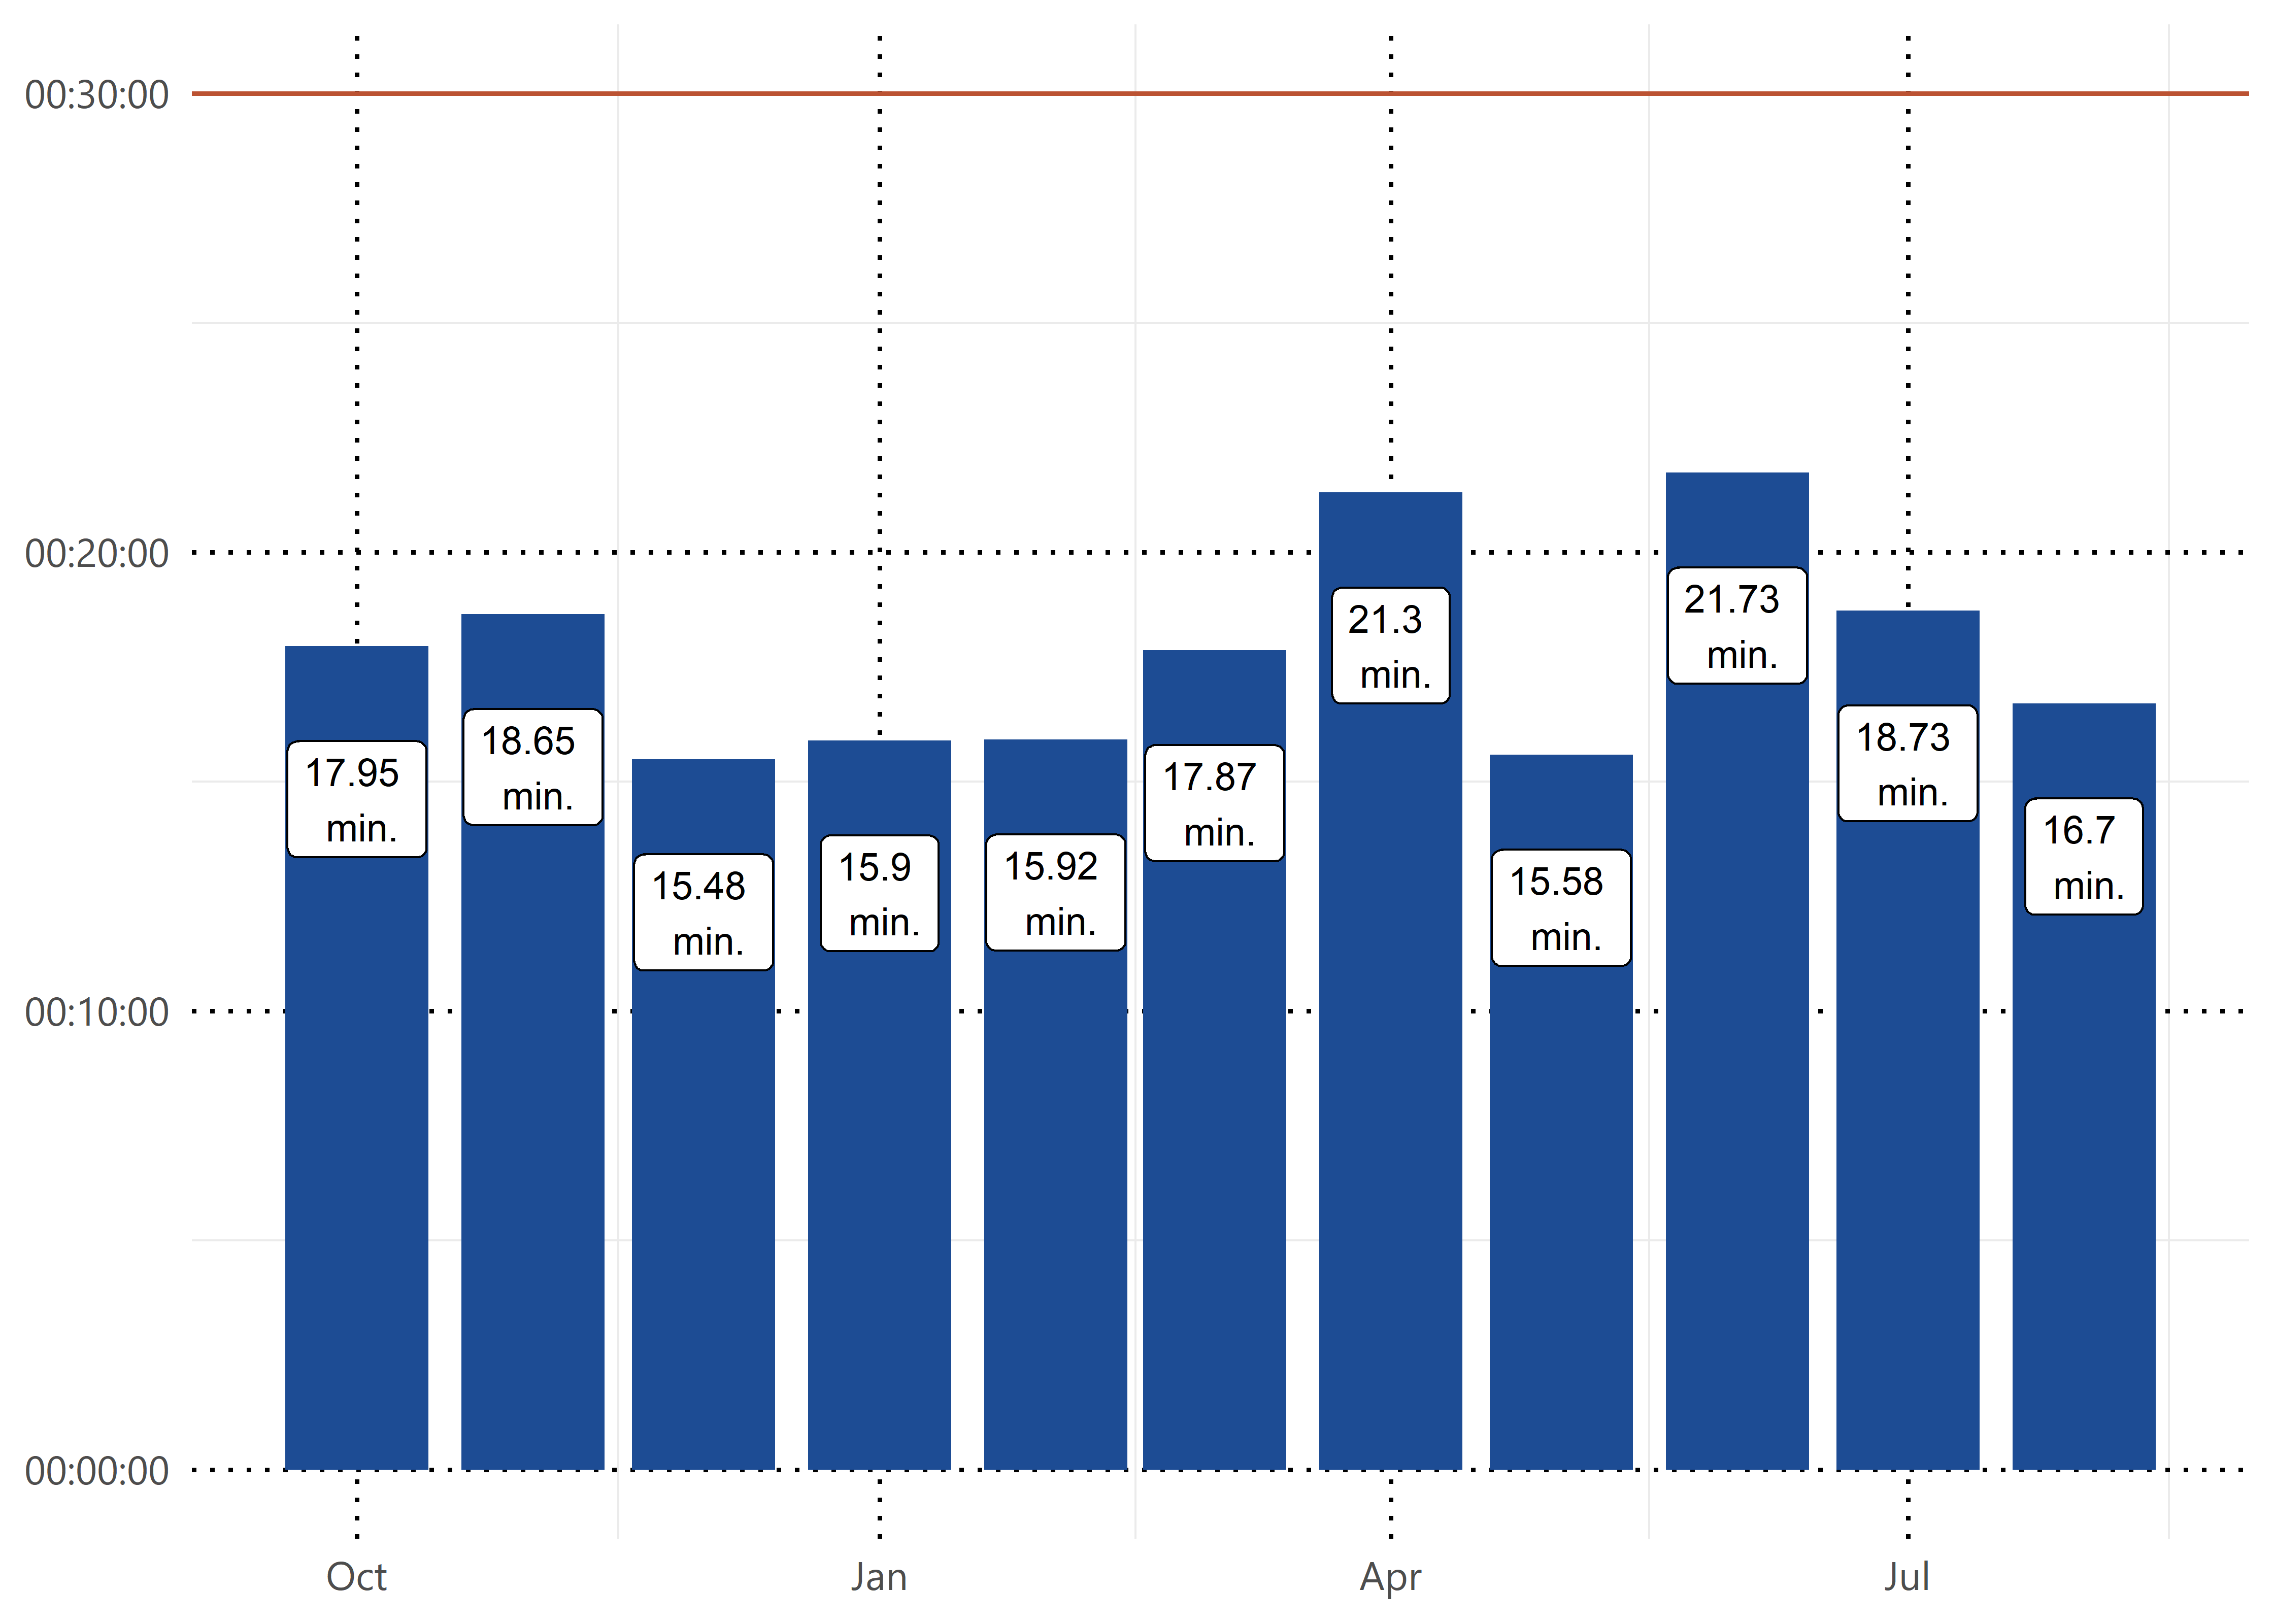
\includegraphics[width=1\linewidth]{bookdown-testing_files/figure-latex/unnamed-chunk-8-1}

\hypertarget{second-priority-call-volume}{%
\section{Second Priority Call Volume}\label{second-priority-call-volume}}

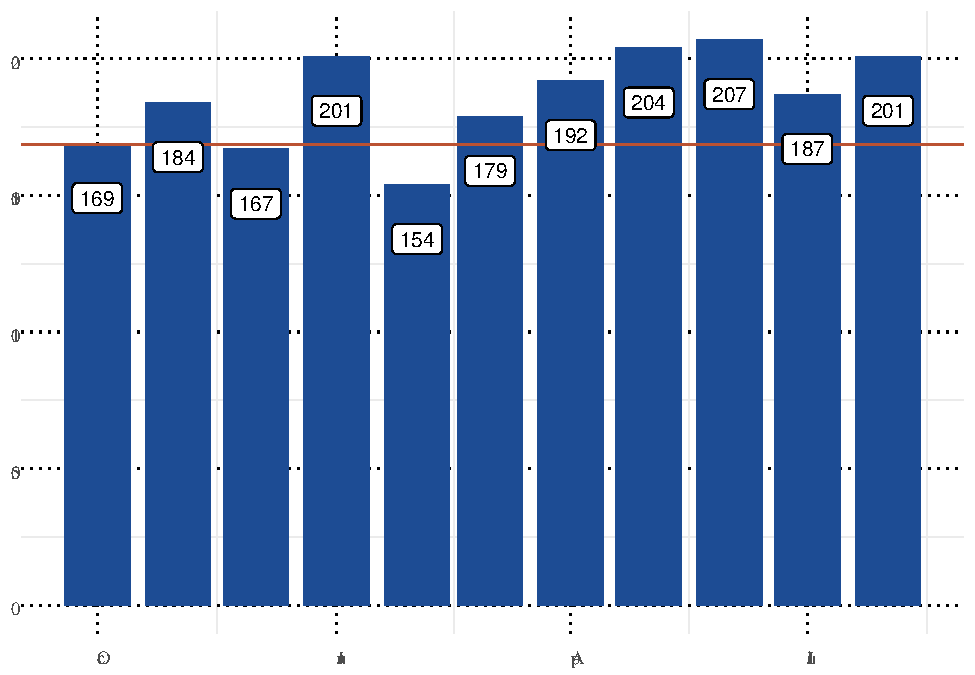
\includegraphics[width=1\linewidth]{bookdown-testing_files/figure-latex/unnamed-chunk-9-1}

\hypertarget{second-priority-average-response-time}{%
\section{Second Priority Average Response Time}\label{second-priority-average-response-time}}

Average response time against our established 60 minute target (not shown).

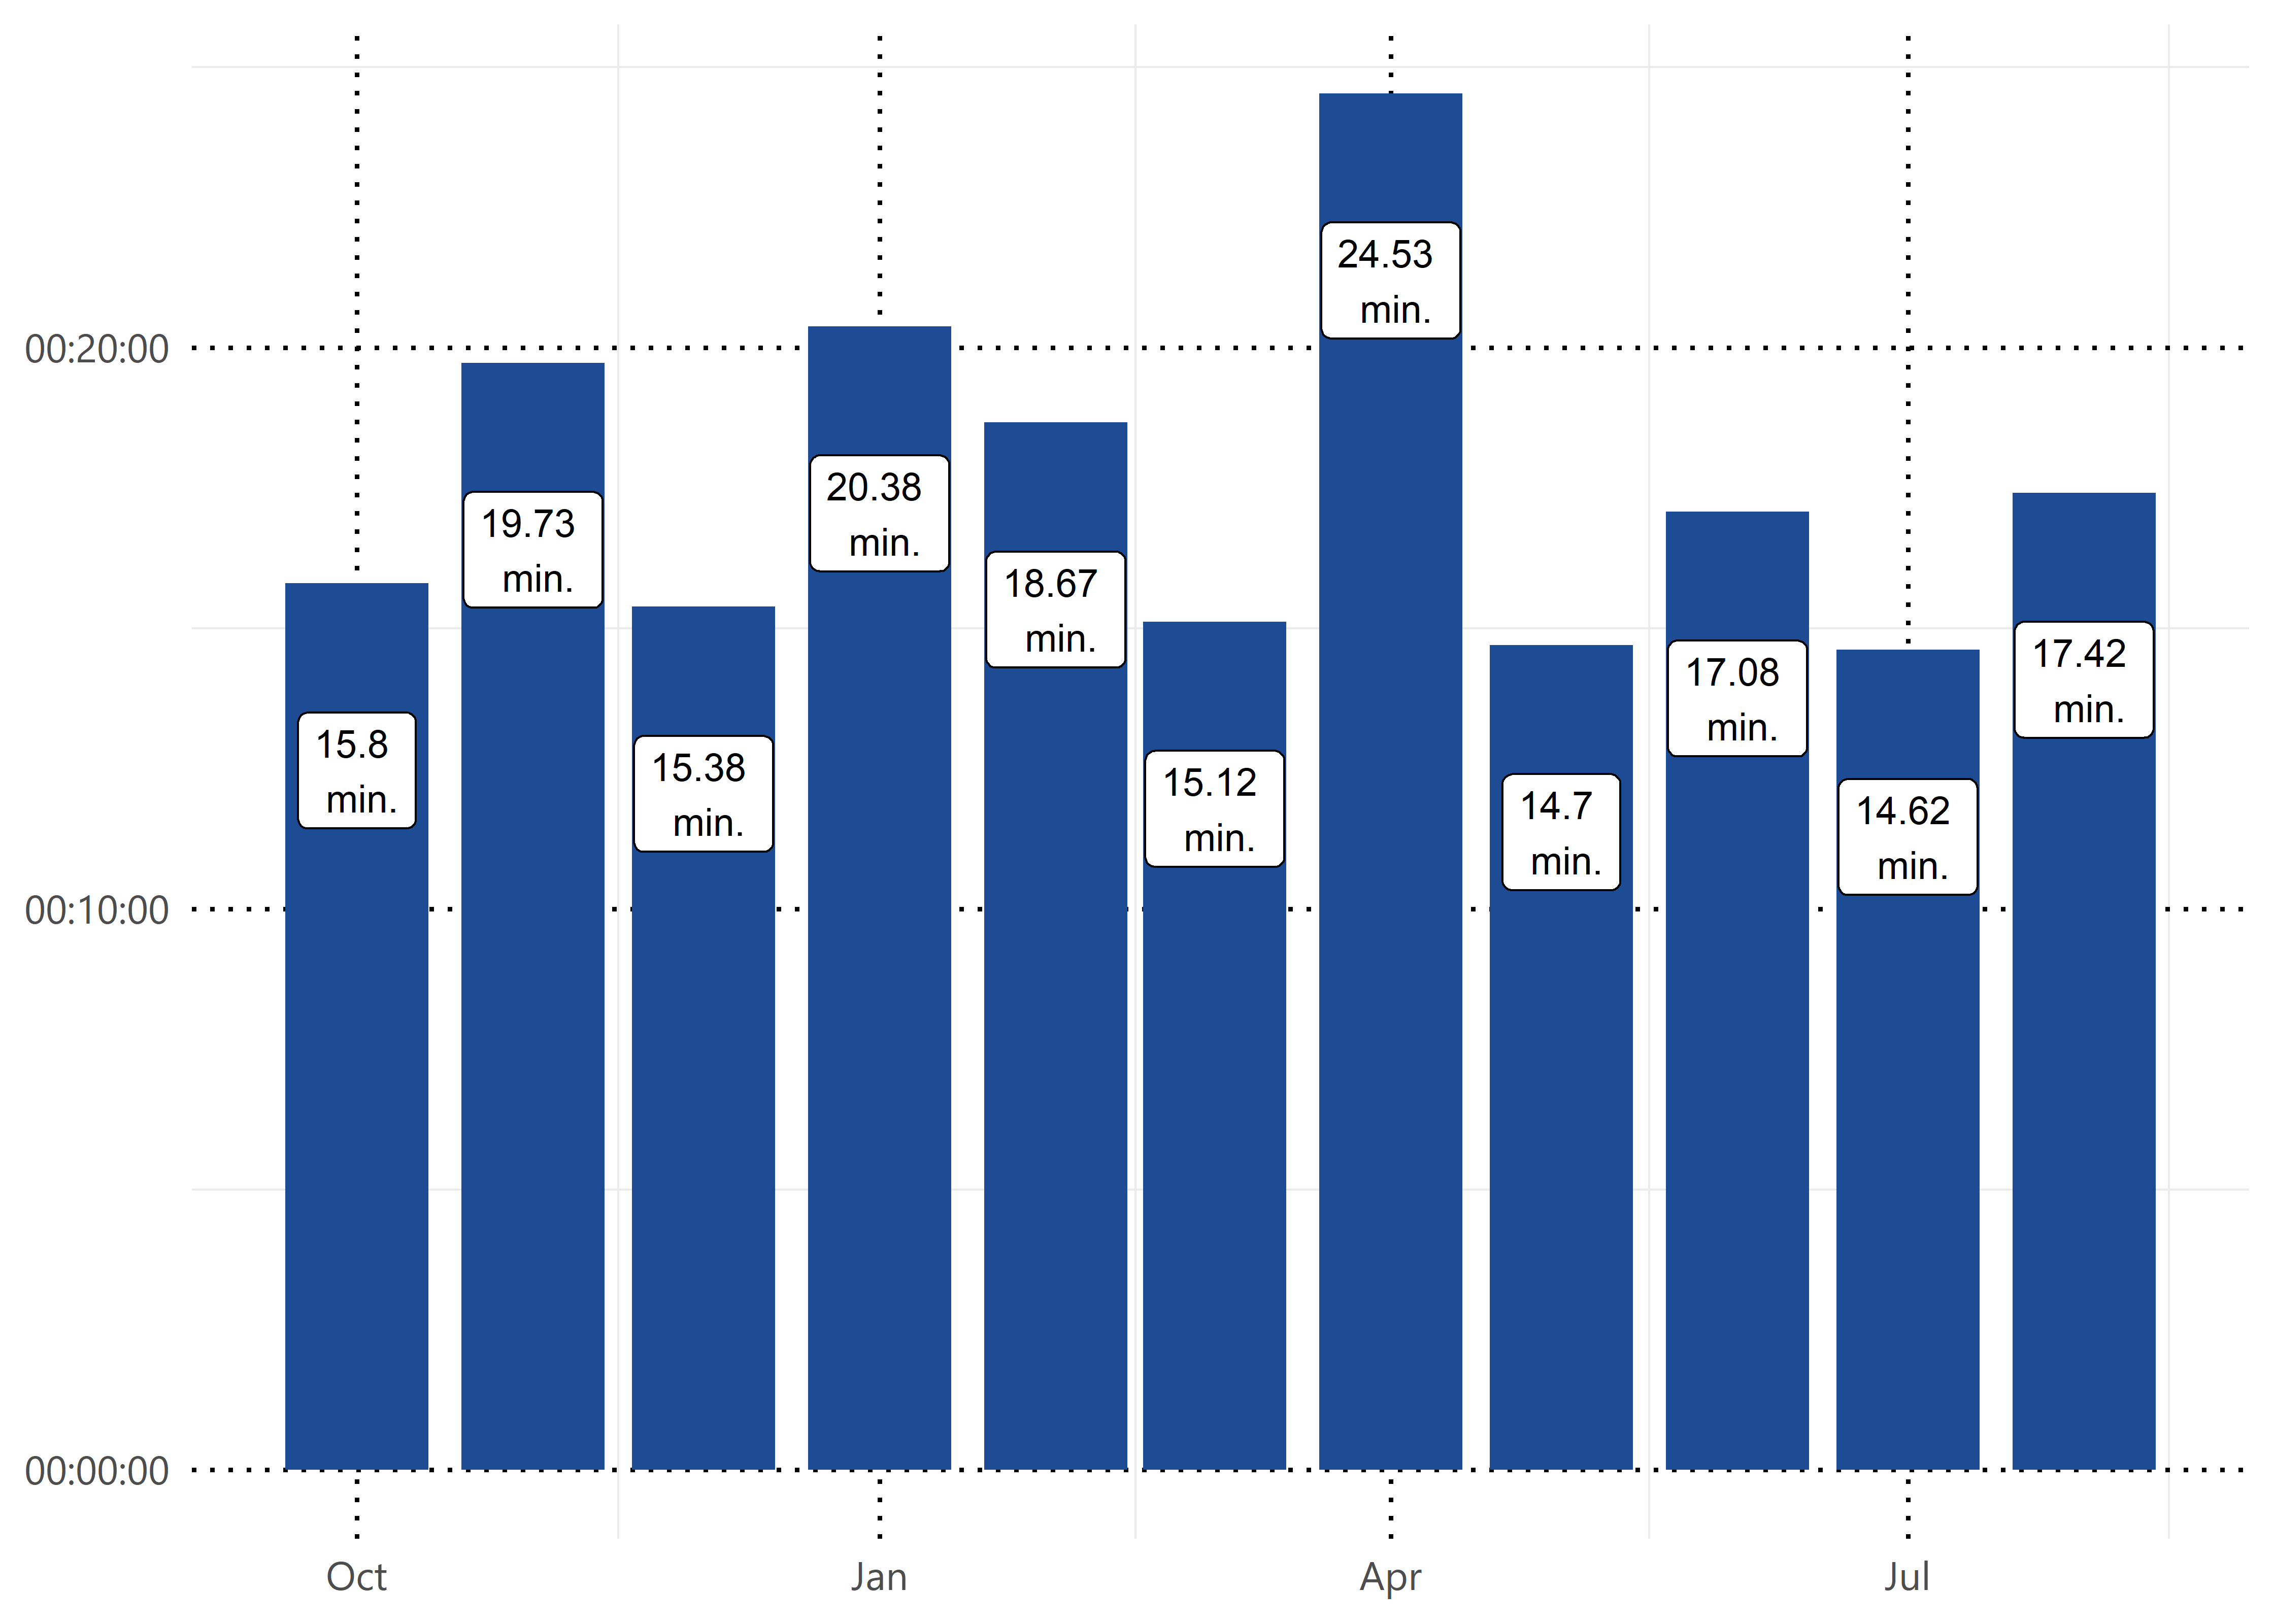
\includegraphics[width=1\linewidth]{bookdown-testing_files/figure-latex/unnamed-chunk-10-1}

\hypertarget{third-priority-call-volume}{%
\section{Third Priority Call Volume}\label{third-priority-call-volume}}

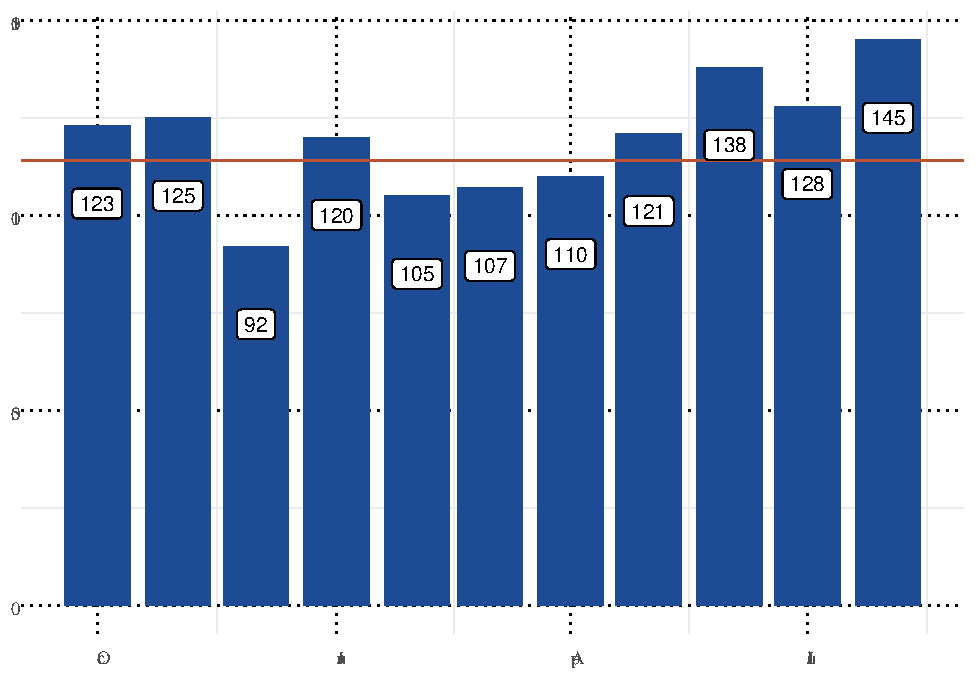
\includegraphics[width=1\linewidth]{bookdown-testing_files/figure-latex/unnamed-chunk-11-1}

\hypertarget{third-priority-average-response-time}{%
\section{Third Priority Average Response Time}\label{third-priority-average-response-time}}

Average response time against our established 90 minute target (not shown).

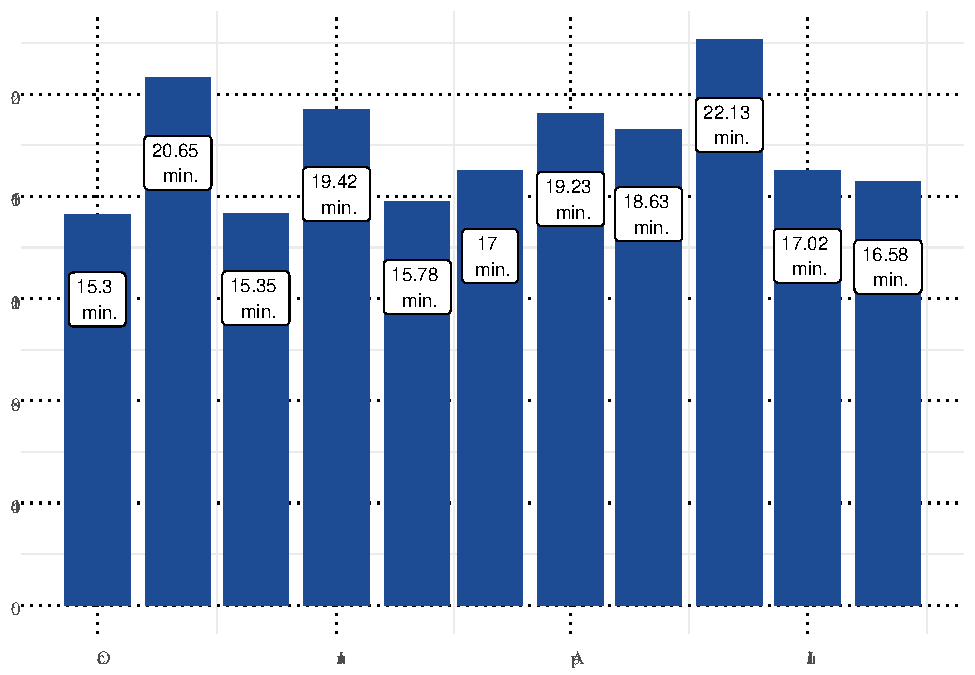
\includegraphics[width=1\linewidth]{bookdown-testing_files/figure-latex/unnamed-chunk-12-1}

\hypertarget{all-other-priority-call-volume}{%
\section{All Other Priority Call Volume}\label{all-other-priority-call-volume}}

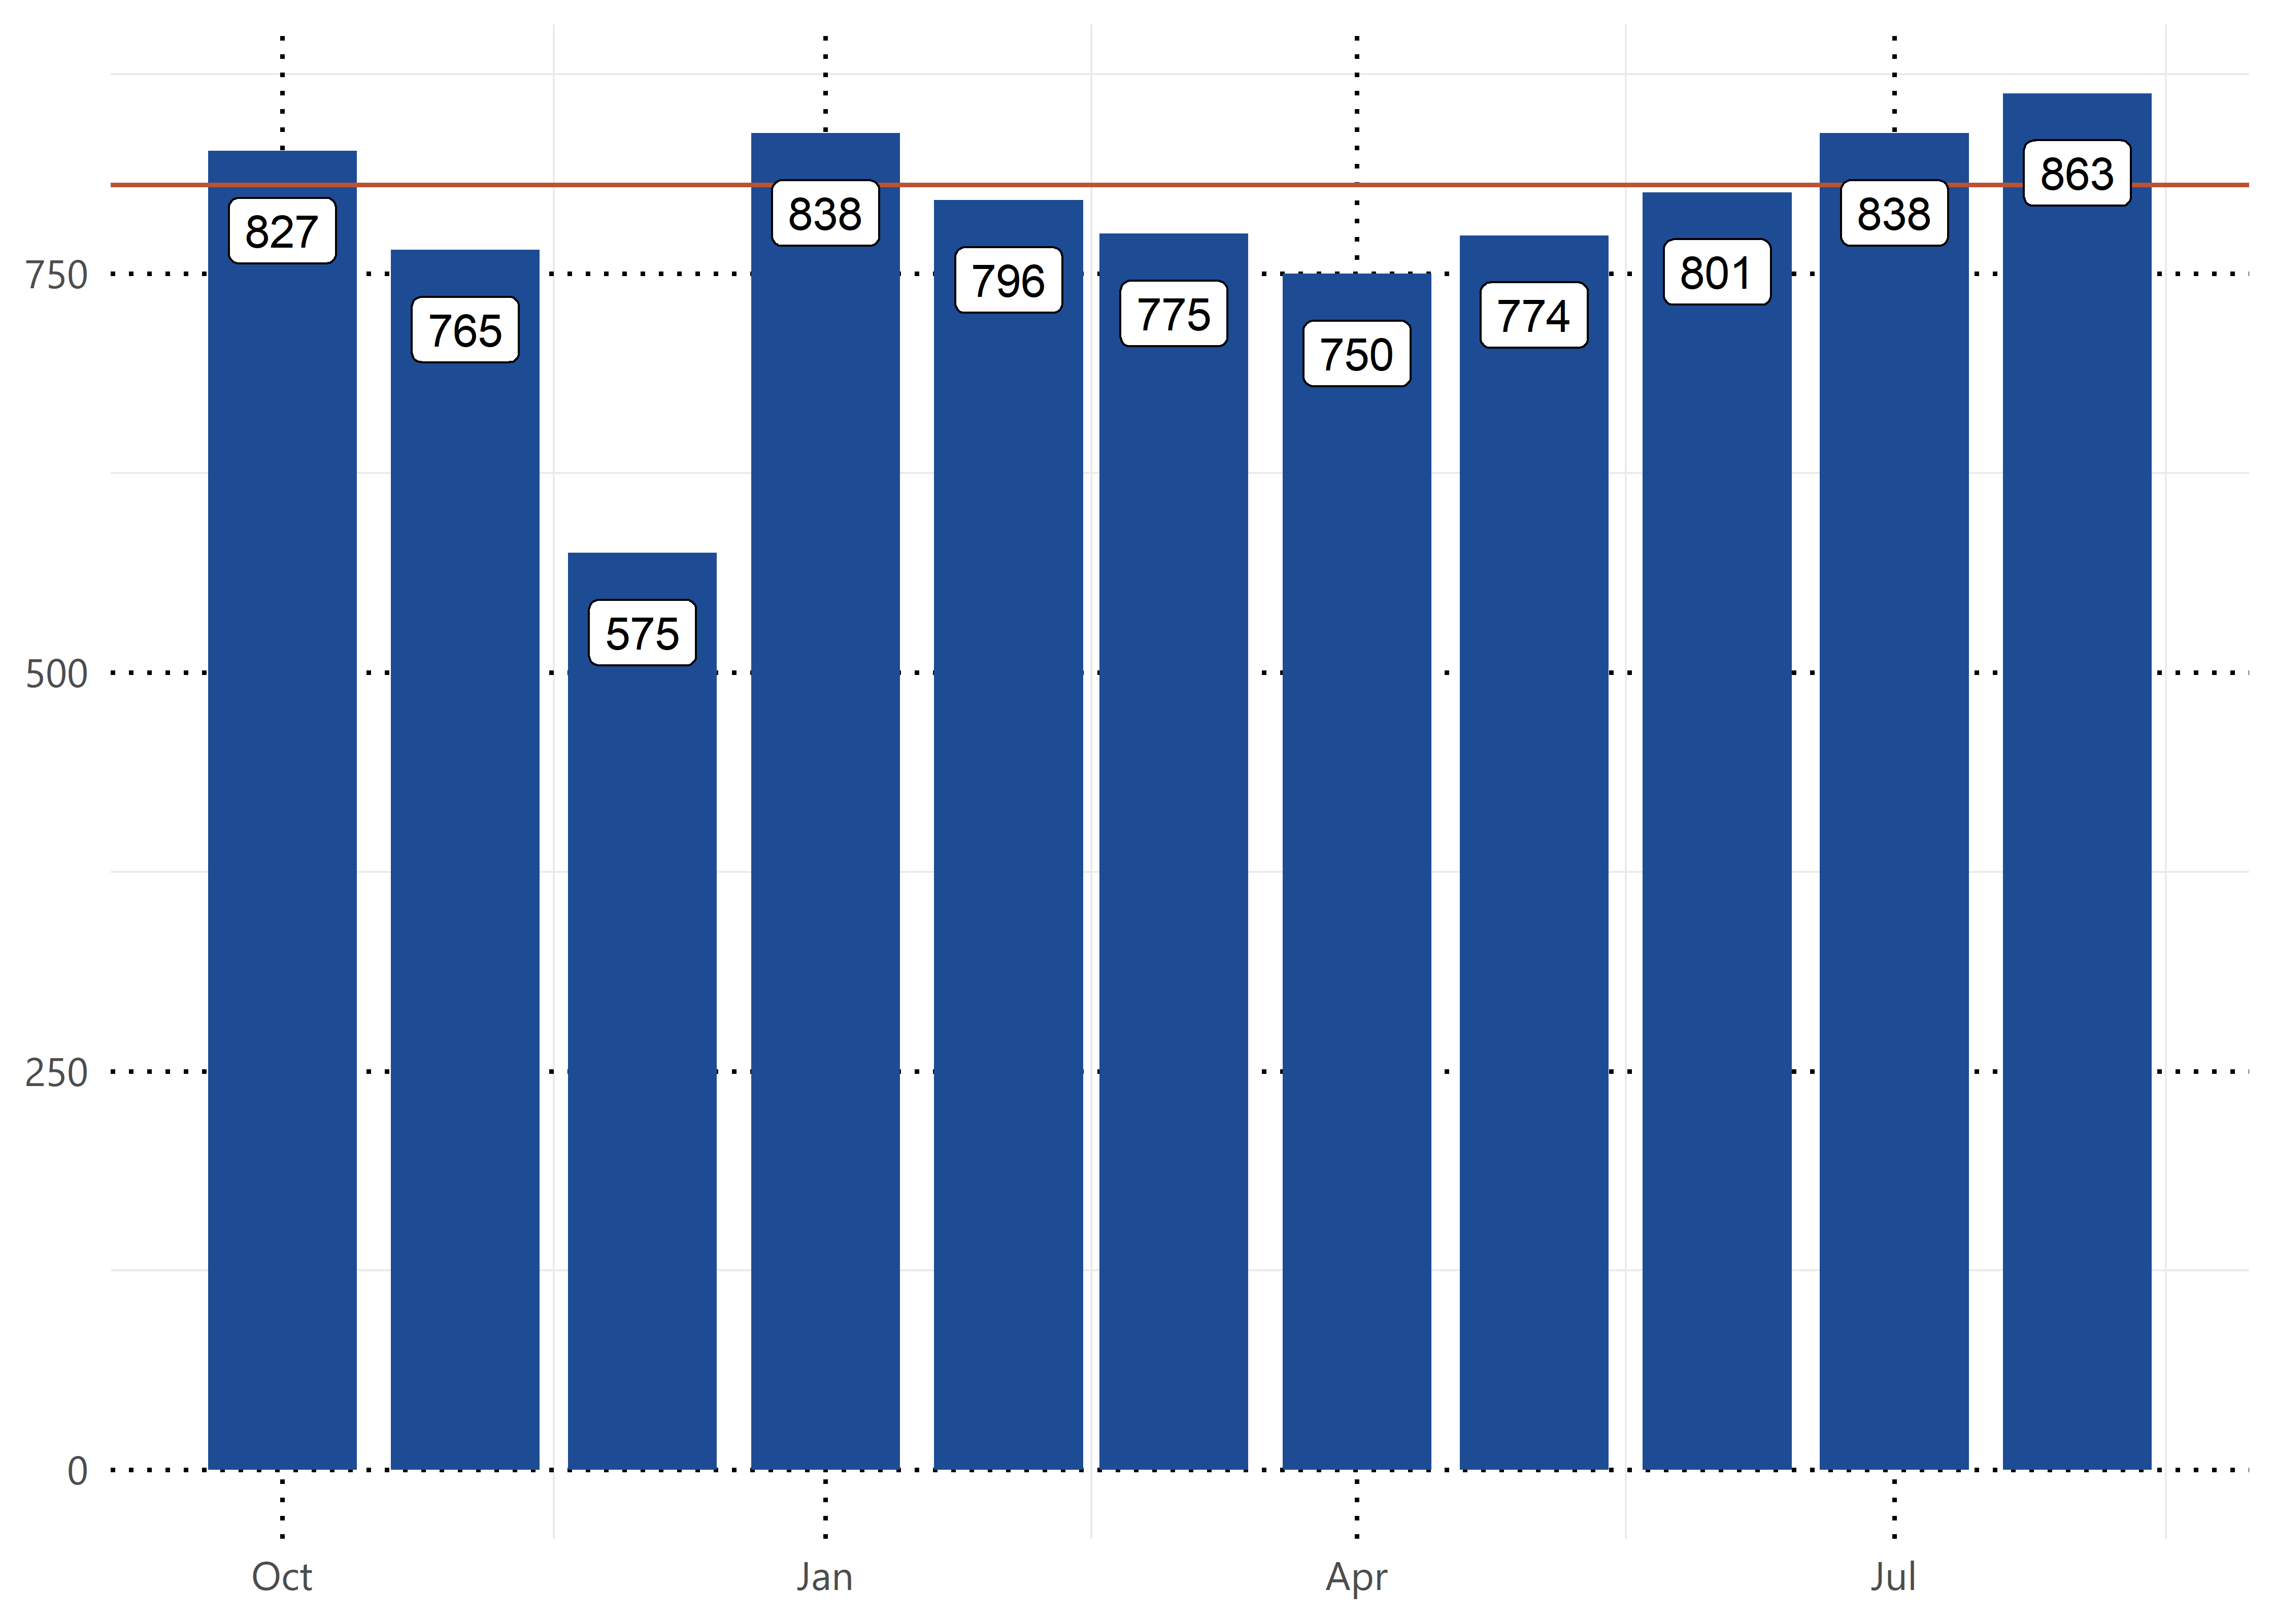
\includegraphics[width=1\linewidth]{bookdown-testing_files/figure-latex/unnamed-chunk-13-1}

\hypertarget{all-other-priority-average-response-time}{%
\section{All Other Priority Average Response Time}\label{all-other-priority-average-response-time}}

Average response time against our established 120 minute target (not shown).

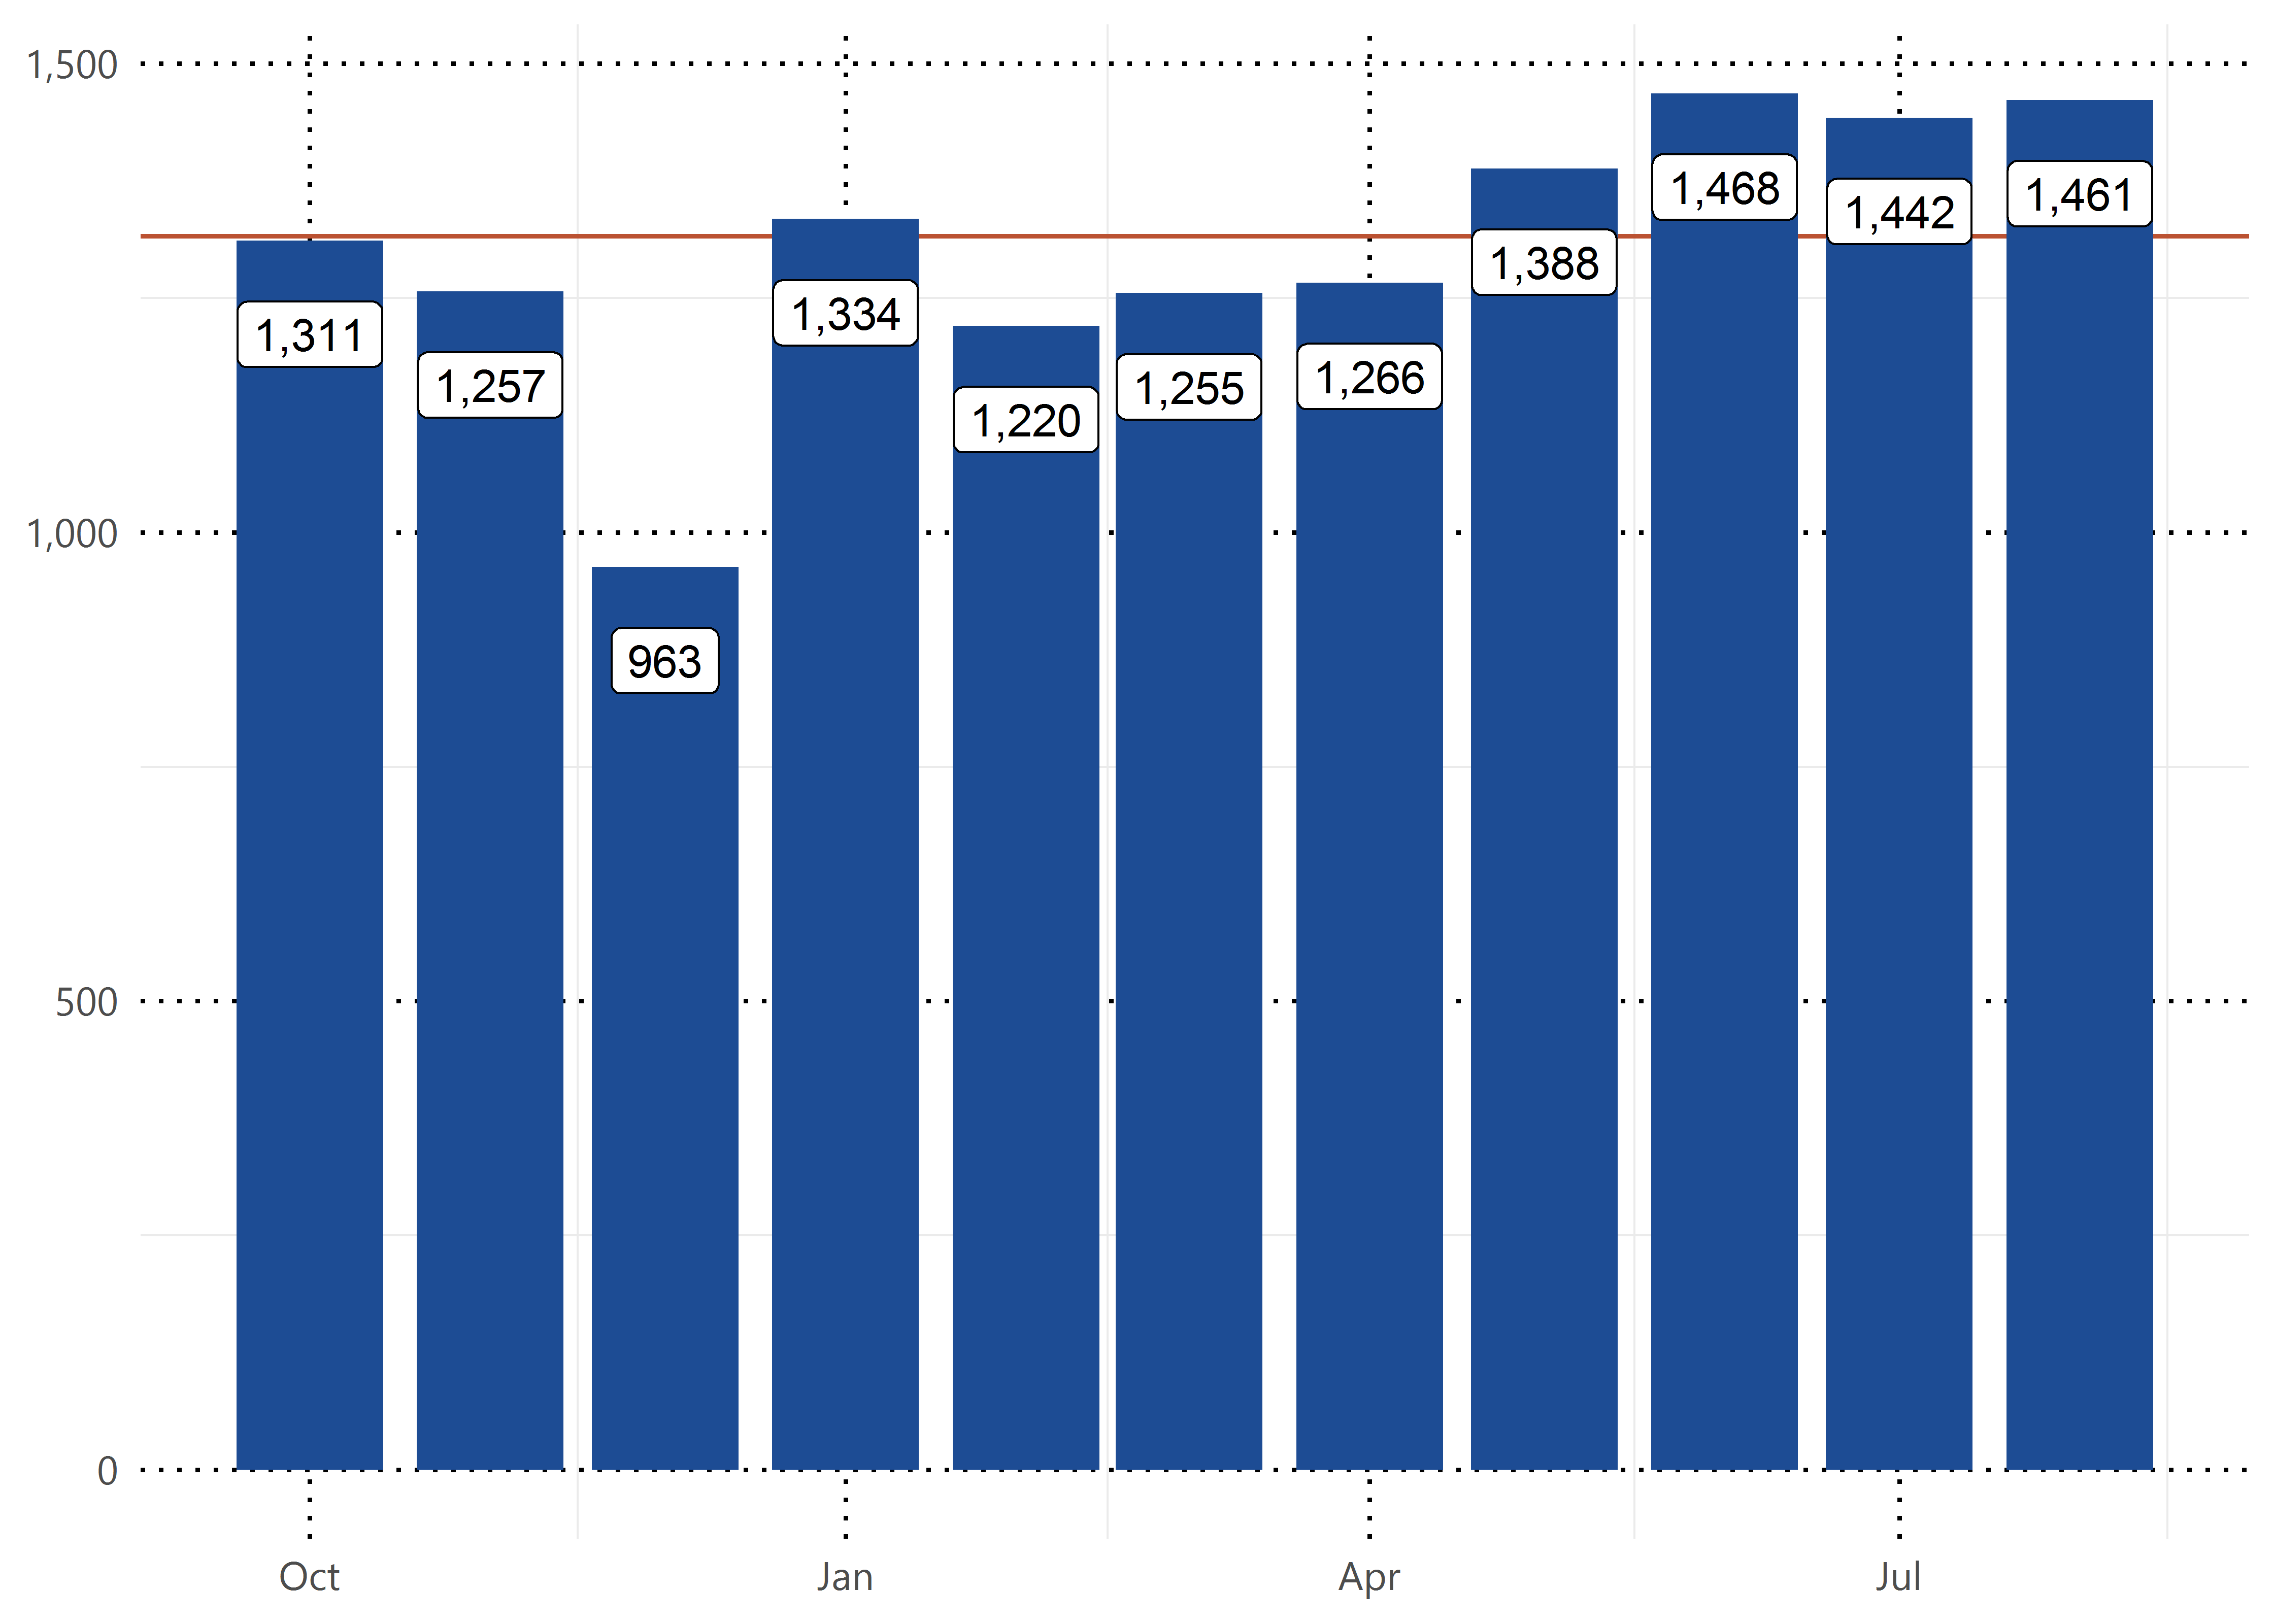
\includegraphics[width=1\linewidth]{bookdown-testing_files/figure-latex/unnamed-chunk-14-1}

\hypertarget{ems}{%
\chapter{Emergency Services}\label{ems}}

Guilford County Emergency Services strives to provide the highest standards of service to
everyone who lives, works or visits the County in the areas of Fire and Life Safety Services,
Emergency Medical Services (EMS), Emergency Management, Fire Inspections and
Investigations, and Fire/Hazardous Materials response. Additionally, the Department operates a
Public Safety
Maintain safe and secure communities through strategically coordinated and
professional public safety services.
133
self-contained Fleet Maintenance Facility to assure that all vehicles and equipment in the various
divisions are available for immediate response to the maximum extent possible.

\hypertarget{emsmonthlycallvolume}{%
\section{Monthly Call Volume}\label{emsmonthlycallvolume}}

How many calls does EMS answer each month?

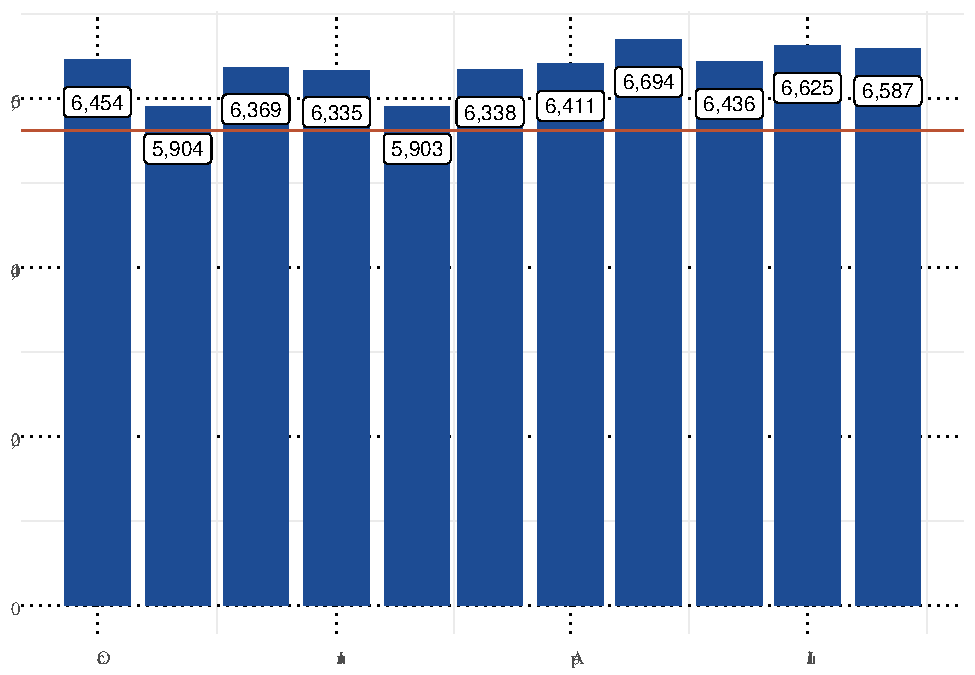
\includegraphics[width=1\linewidth]{bookdown-testing_files/figure-latex/unnamed-chunk-16-1}

\hypertarget{emsyearlycallvolume}{%
\section{Yearly Call Volume}\label{emsyearlycallvolume}}

How many calls do we receive each fiscal year?

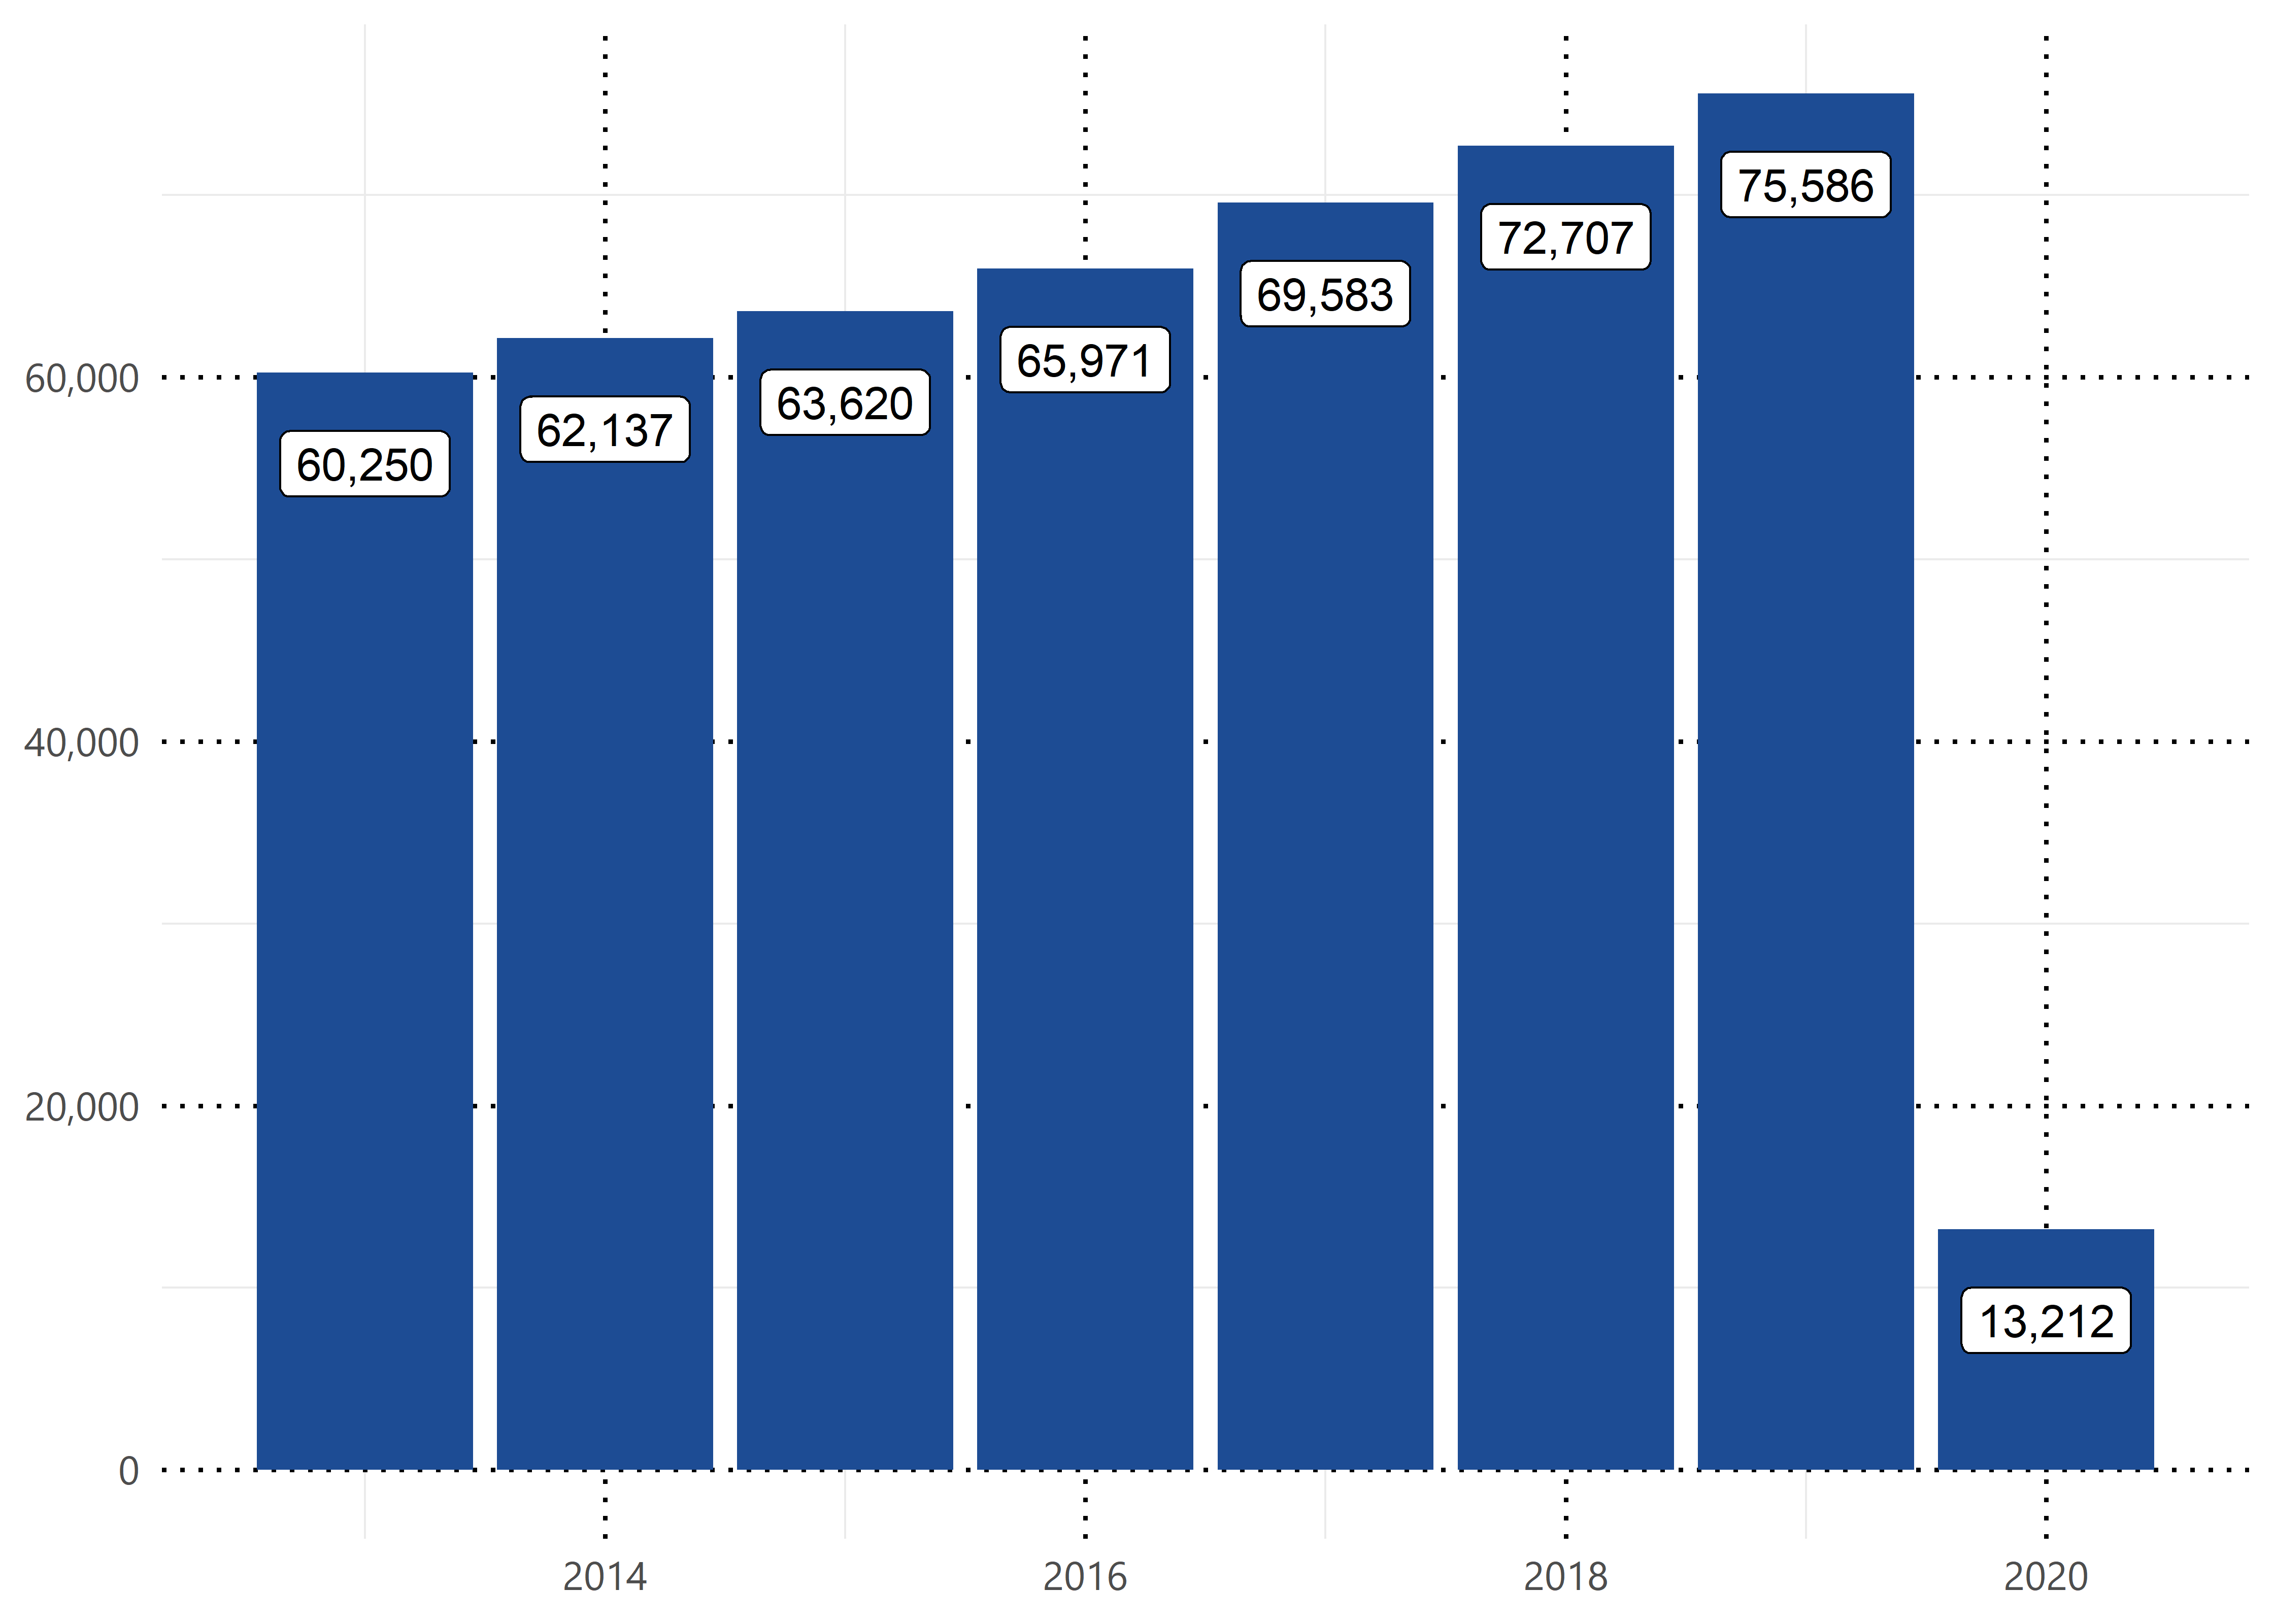
\includegraphics[width=1\linewidth]{bookdown-testing_files/figure-latex/unnamed-chunk-17-1}

\hypertarget{emsoverallavgresp}{%
\section{Overall Average Response Time}\label{emsoverallavgresp}}

This is the overall average response time for all calls and priorities.

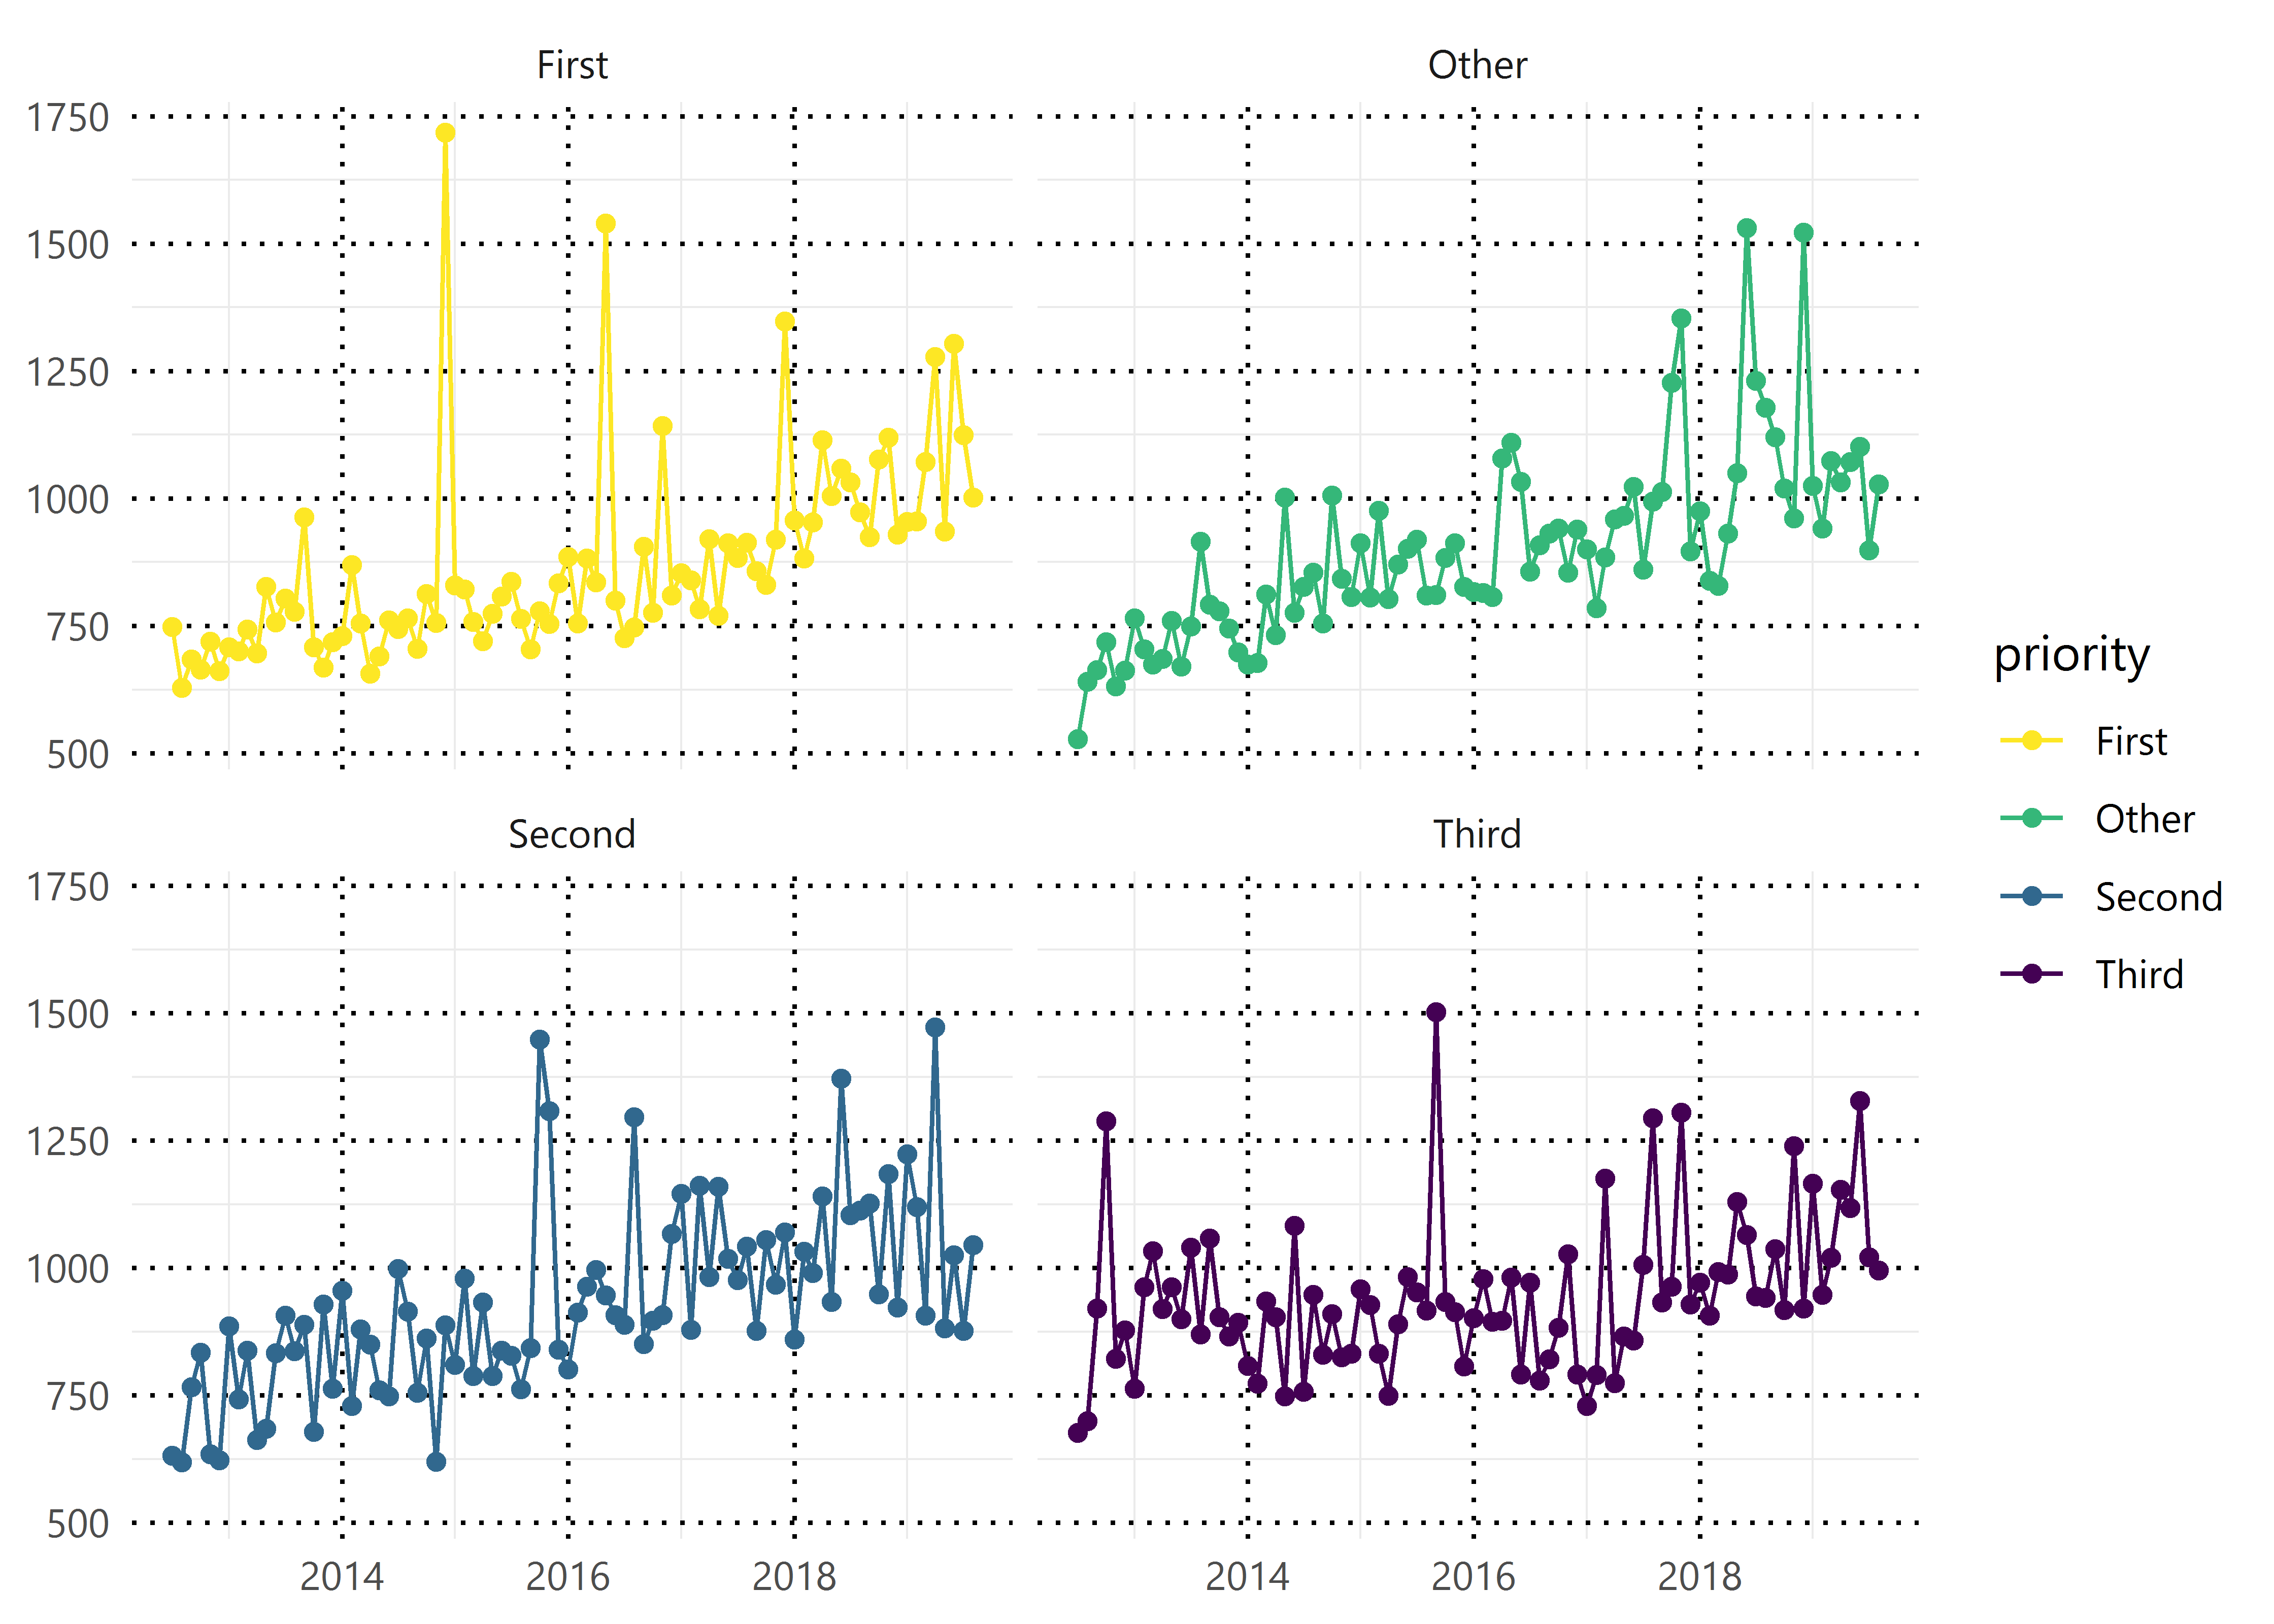
\includegraphics[width=1\linewidth]{bookdown-testing_files/figure-latex/unnamed-chunk-18-1}

\hypertarget{priority-breakdown-1}{%
\section*{Priority Breakdown}\label{priority-breakdown-1}}
\addcontentsline{toc}{section}{Priority Breakdown}

\hypertarget{imminent-life-threat}{%
\section{Imminent Life Threat}\label{imminent-life-threat}}

Goal is to arrive in under 9 minutes, 90\% of the time.

\hypertarget{emsimcallcount}{%
\section{Imminent Life Threat Call Count}\label{emsimcallcount}}

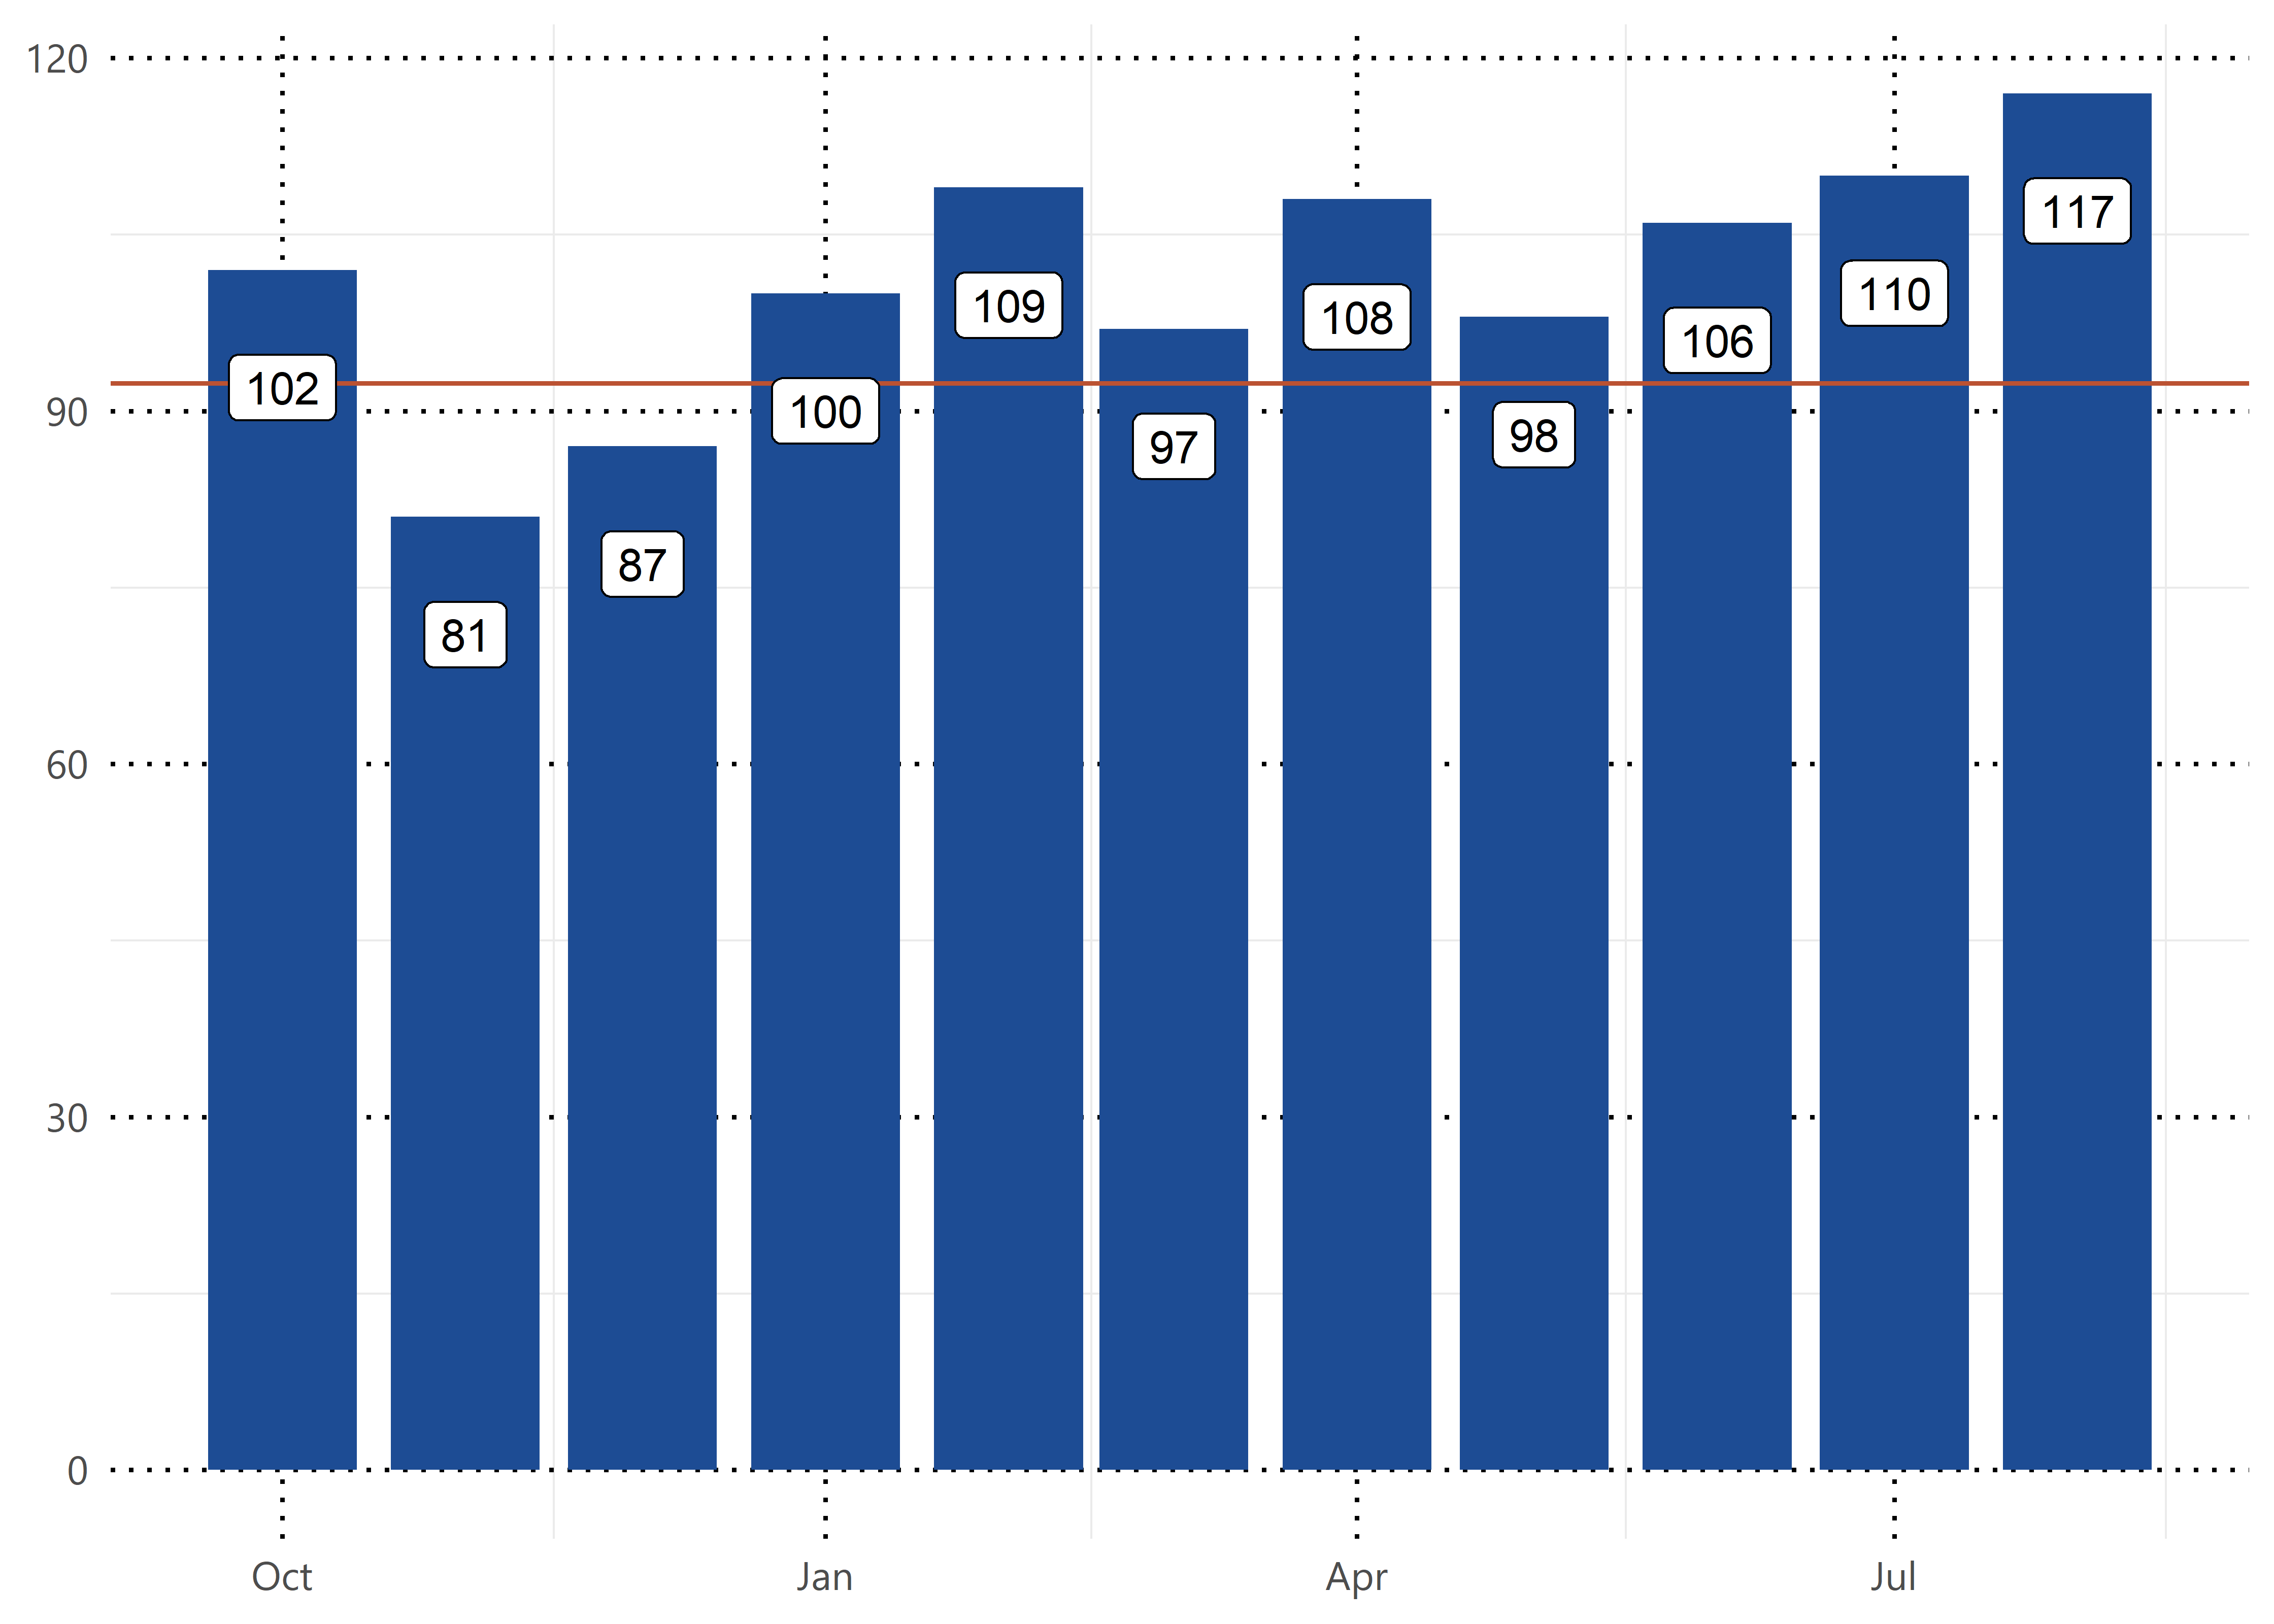
\includegraphics[width=1\linewidth]{bookdown-testing_files/figure-latex/unnamed-chunk-19-1}

\hypertarget{emsimavgresp}{%
\section{Imminenet Life Threat Average Response Time}\label{emsimavgresp}}

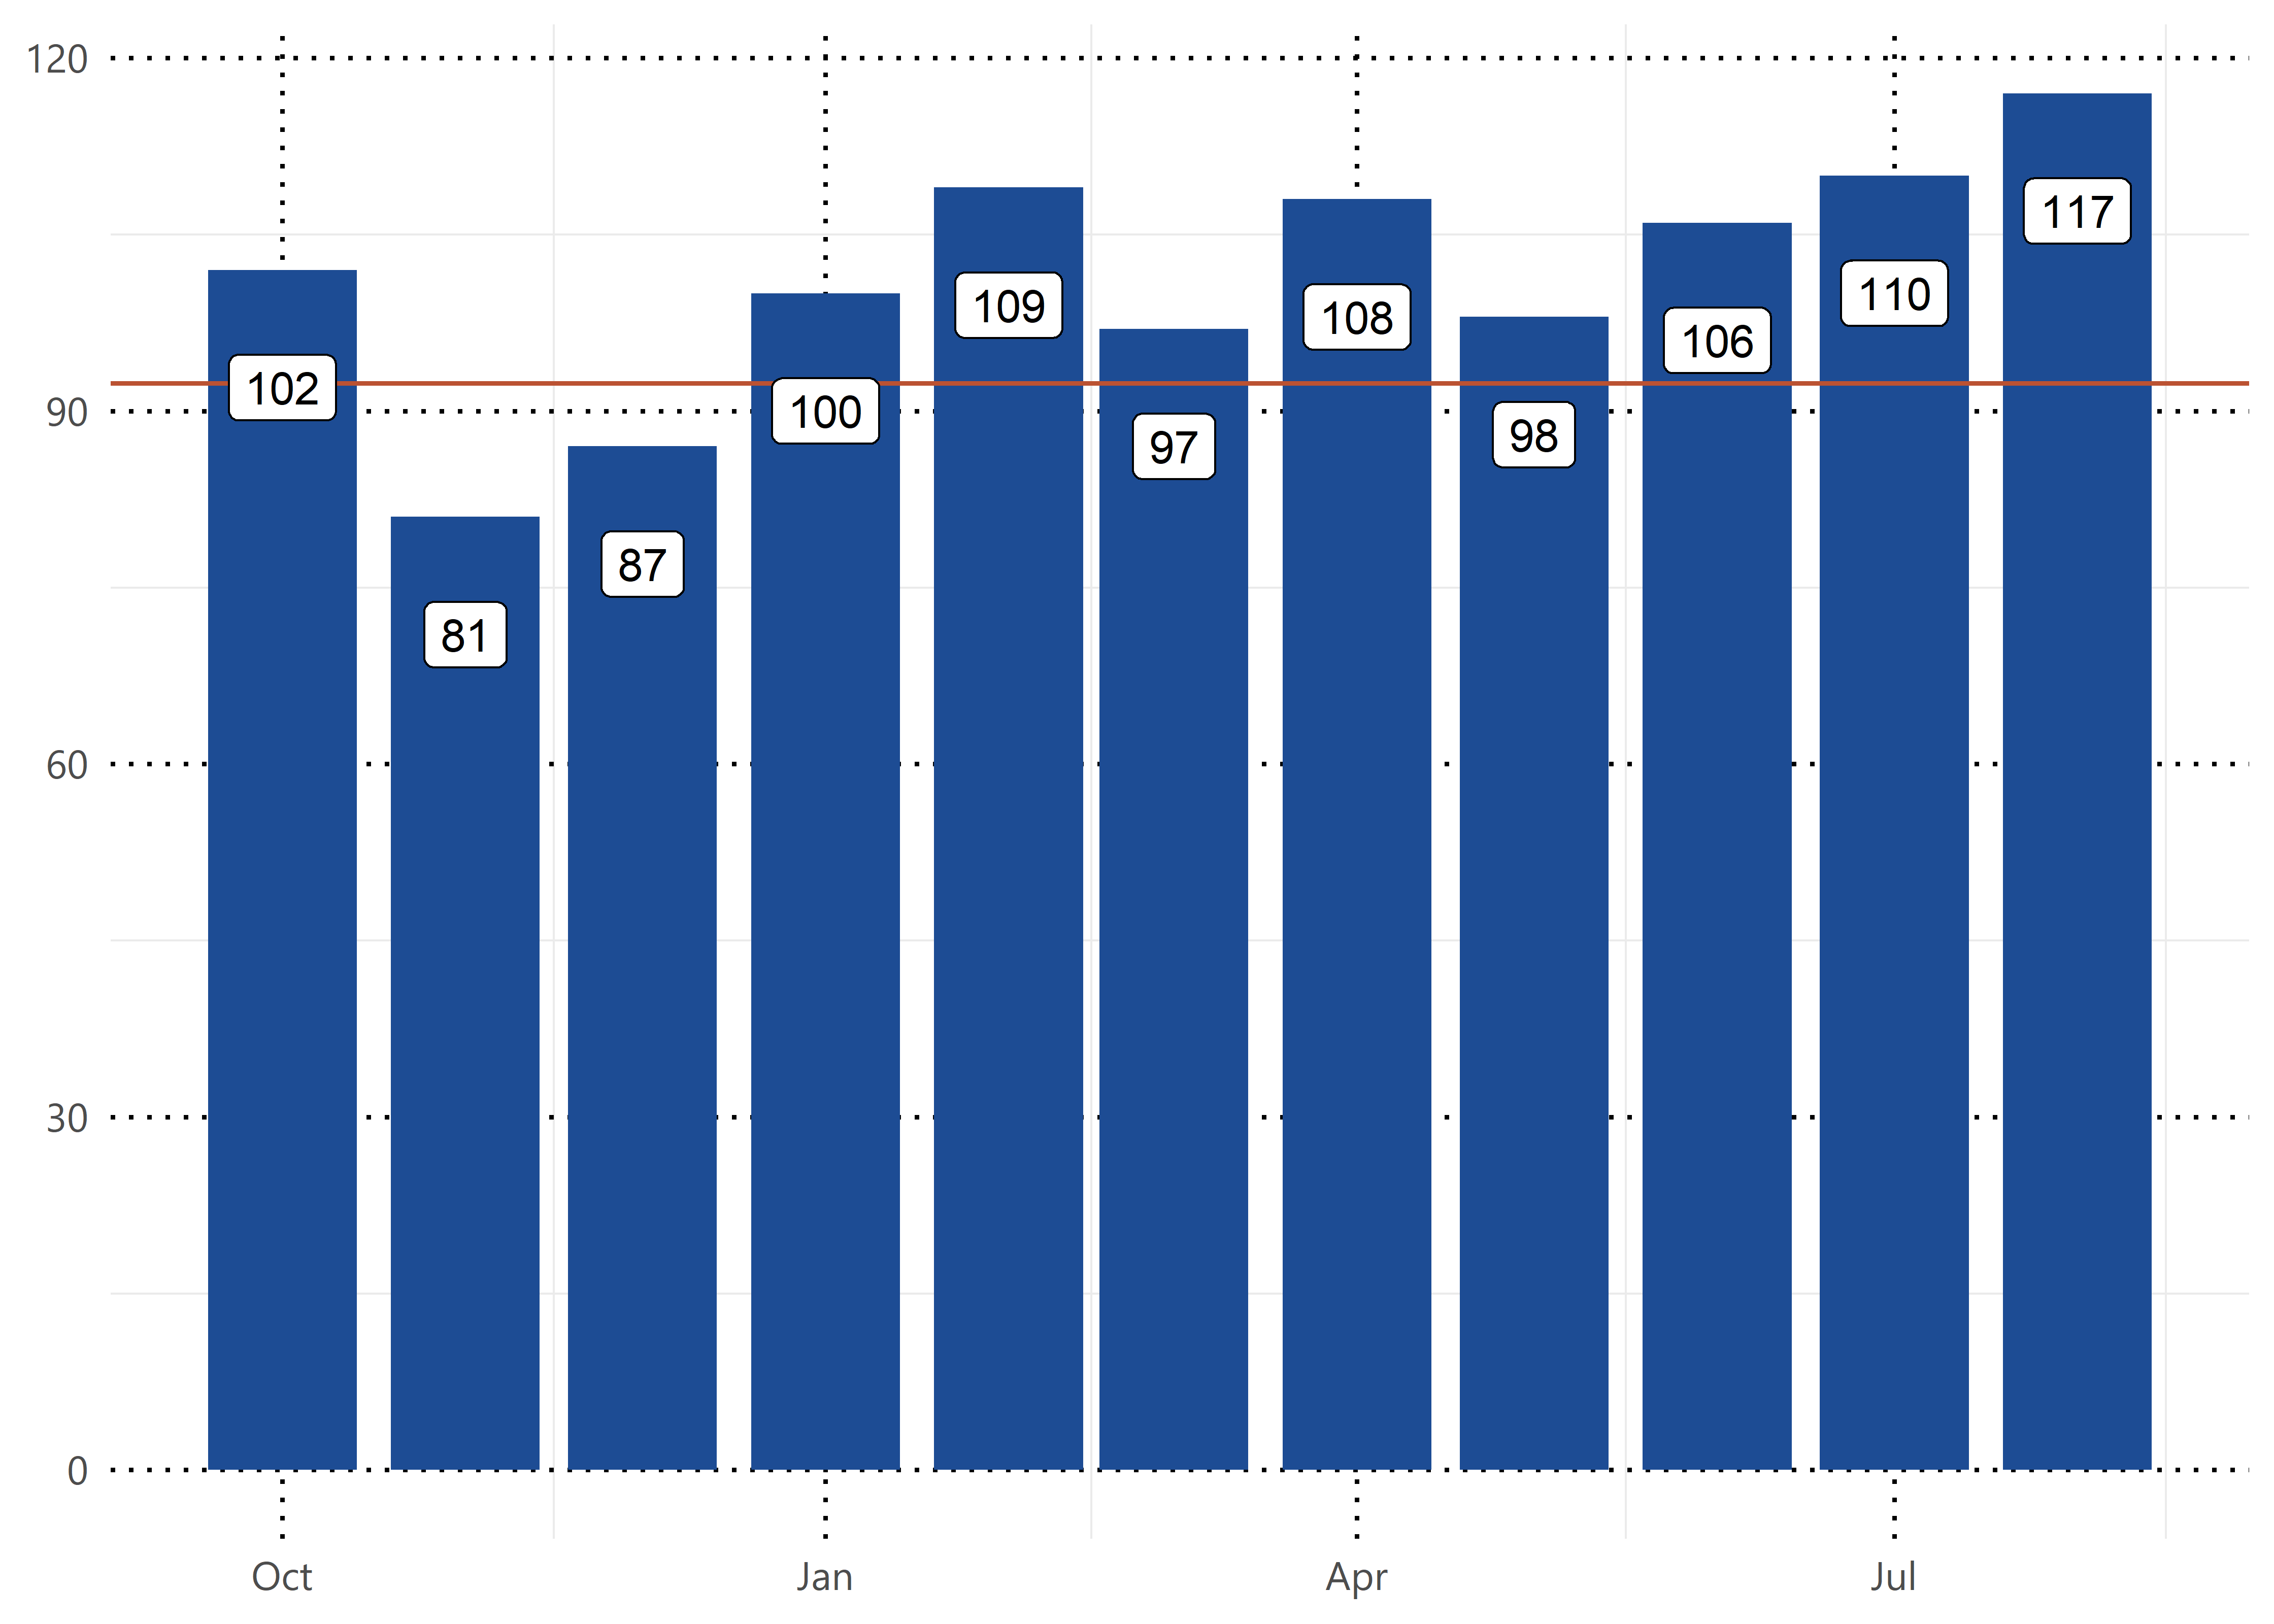
\includegraphics[width=1\linewidth]{bookdown-testing_files/figure-latex/unnamed-chunk-20-1}

\hypertarget{emsimpercunder}{%
\section{Imminenet Life Threat Percent Under}\label{emsimpercunder}}

What percent of the time did we arrive in under 9 minutes?

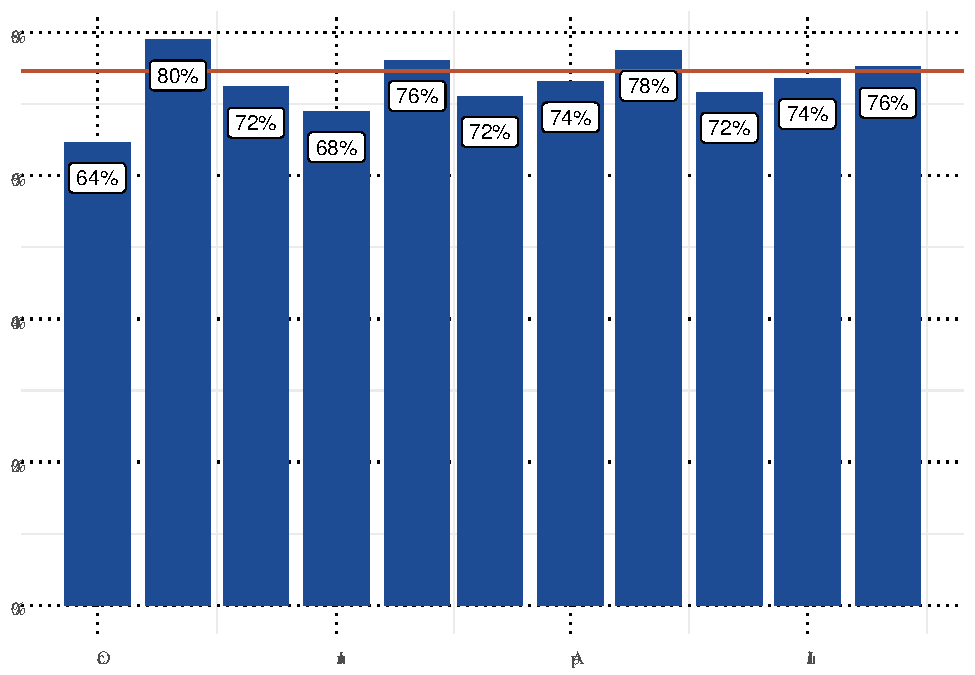
\includegraphics[width=1\linewidth]{bookdown-testing_files/figure-latex/unnamed-chunk-21-1}

\bibliography{book.bib,packages.bib}


\end{document}
